\mbox{}\\
\vspace{8cm}

This chapter is a reproduction of the following publication:

A. Friães, R. Mamede, M. Ferreira, J. Melo-Cristino, M. Ramirez, Annotated Whole-Genome Multilocus Sequence Typing Schema for Scalable High-Resolution Typing of \textit{Streptococcus pyogenes}, Journal of Clinical Microbiology, Volume 60, Issue 6, May 2022. DOI: \url{https://doi.org/10.1128/jcm.00315-22}

The supplementary material referred to throughout the text can be consulted in the last section of this chapter, \textbf{\autoref{sec:ch4_supplemental_material}}.

Schemas are the centerpiece of \ac{wg/cgMLST}. A \ac{wg/cgMLST} schema captures the diversity of a set of loci, generally identified in a single bacterial species, and, through allele calling, allows the determination of the allelic profiles of strains of interest. Creating a schema for \ac{wg/cgMLST} is not necessarily complex. Creating a well-curated \ac{wg/cgMLST} schema that captures the diversity of thousands of loci of a bacterial species is a different matter altogether. Well-curated means that all loci or nearly all loci in the schema are \textit{bona fide} loci, not spurious loci, such as frameshifted, truncated, or gene fusions, which are common issues plaguing \ac{wg/cgMLST} schemas. Limiting the set of loci included in the schemas to the core loci to define a \ac{cgMLST} schema is a way to minimize these problems. In theory, \ac{cgMLST} schemas should include loci present in all or nearly all strains of a dataset representative of the diversity of a species, corresponding to loci with more conserved sequences due to their important functions. Although \ac{cgMLST} schemas may provide robust results, in many cases they do not capture a considerable fraction of the diversity of bacterial species, limiting their applicability, such as for high-resolution typing of closely related strains in outbreak contexts. \ac{wgMLST} schemas incorporate loci from the most variable fraction of the genome, usually termed the accessory genome, and provide greater resolution than \ac{cgMLST} schemas. However, creating a \ac{wgMLST} schema is a laborious process, as incomplete genome assemblies, errors derived from genome misassembly, and the dynamic nature of the accessory genome can hinder identification of \textit{bona fide} alleles and blur loci definitions.

This chapter describes the creation of a \ac{wgMLST} schema for high-resolution typing of \textit{Streptococcus pyogenes}. \textit{S. pyogenes} is a major human pathogen that was included in the \ac{WHO} \ac{BPPL} released in 2024 due to reports of increased resistance to macrolides. Following the creation of a schema seed based on a set of high-quality complete genomes with an early version of chewBBACA 3, presented in \textbf{\autoref{ch:paper1}}, the schema was populated with alleles identified in several datasets representing the known diversity of \textit{S. pyogenes}. The schema was then extensively annotated through automatic methods, followed by curation by the first first co-author, an expert in the biology of \textit{S. pyogenes}, to validate the annotations and identify spurious loci. The schema was refined to remove or substitute spurious loci by valid alleles. The refinement resulted in a final \ac{wg/cgMLST} schema with 3,044 loci, which captures far more of the diversity of \textit{S. pyogenes} than the computed \ac{cgMLST} schemas, which include only between 763 and 1321 loci. Using a \ac{wgMLST} schema instead of hard-defined \ac{cgMLST} schemas allows adjusting \ac{cgMLST} analyses dynamically for each dataset, identifying more loci than conventional \ac{cgMLST} and achieving performance comparable to \ac{SNP}-based methods.

I participated in all steps related to schema development and dataset analyses to evaluate schema performance. Throughout the schema development process, I was responsible for selecting the genomes used for schema creation, annotating the schema loci based on multiple sources, and refining the schema based on the suggestions of the first first co-author. When necessary, I implemented custom scripts to annotate, refine, and evaluate schema performance.

\newpage 

\begin{center}
\large
\textbf{Annotated Whole-Genome Multilocus Sequence Typing Schema for Scalable High-Resolution Typing of \textit{Streptococcus pyogenes}}
\end{center}

Ana Friães$^{1,*}$, 
Rafael Mamede$^{1,*}$, 
Mariana Ferreira$^1$,
José Melo-Cristino$^1$, 
Mário Ramirez$^1$,

$^1$Instituto de Microbiologia, Instituto de Medicina Molecular, Faculdade de Medicina, Universidade de Lisboa, Lisboa, Portugal 

$^*$Contributed equally

\section{Abstract} \label{sec:ch4_abstract}

\textit{Streptococcus pyogenes} is a major human pathogen with high genetic diversity, largely created by recombination and horizontal gene transfer, making it difficult to use \ac{SNP}-based genome-wide analyses for surveillance. Using a Gene-by-Gene approach on 208 complete genomes of \textit{S. pyogenes}, a novel \ac{wgMLST} schema was developed, comprising 3,044 target loci. The schema was used for \ac{cgMLST} analyses of previously published data sets and 265 newly sequenced draft genomes with other molecular and phenotypic typing data. Clustering based on \ac{cgMLST} data supported the genetic heterogeneity of many \textit{emm} types and correlated poorly with \ac{PFGE} macrorestriction profiling, superantigen gene profiling, and \ac{MLST} sequence type, highlighting the limitations of older typing methods. While 763 loci were present in all isolates of a data set representative of \textit{S. pyogenes} genetic diversity, the proposed schema allows scalable \ac{cgMLST} analysis, which can include more loci for an increased resolution when typing closely related isolates. The \ac{cgMLST} and PopPUNK clusters were broadly consistent in this diverse population. The \ac{cgMLST} analyses presented results comparable to those of \ac{SNP}-based methods in the identification of two recently emerged sublineages of \textit{emm1} and \textit{emm89} and the clarification of the genetic relatedness among isolates recovered in outbreak contexts. The schema was thoroughly annotated and made publicly available on the \ac{Chewie-NS} online platform (\url{https://chewbbaca.online/species/1/schemas/1}), providing a framework for high-resolution typing and analyzing the genetic variability of loci of particular biological interest.

\section{Introduction} \label{sec:ch4_introduction}

\textit{Streptococcus pyogenes} (\ac{GAS}) remains a significant cause of global morbidity and ranks among the top 10 infectious causes of death \cite{carapetis_global_2005}. In 2018, the \ac{WHO} highlighted the importance of developing a \ac{GAS} vaccine and set out priority activities to reach this goal, including a better characterization of the epidemiology of \ac{GAS} infections and the identification of appropriate candidate antigens \cite{vekemans_path_2019}.

In recent decades, sequence-based typing of the hypervariable region of the \textit{emm} gene, encoding the M protein, was the most frequently used method to identify \ac{GAS} lineages \cite{beall_sequencing_1996}. However, complementary methods have long been used, which, together with \textit{emm} typing, allow finer discrimination of the circulating strains, including serotyping of the major backbone pilus protein (T antigen), \ac{PFGE} macrorestriction profiling, \ac{MLST}, and profiling of superantigen (SAg)-coding genes \cite{carrico_illustration_2006, friaes_superantigen_2013, enright_multilocus_2001}.

\ac{WGS} analysis allowed the identification of emerging intra-\textit{emm} clones with increased fitness or virulence that were otherwise indistinguishable by other typing methods. Such is the case of \textit{emm}89 clade 3, which emerged during the 2000s and quickly outcompeted other emm89 lineages \cite{friaes_emergence_2015, turner_emergence_2015, zhu_molecular_2015}. Isolates from this lineage lack the genes encoding hyaluronic acid capsule biosynthesis and carry a high-expression promoter in the operon encoding streptolysin O and NAD-glycohydrolase (Pnga-3) \cite{turner_emergence_2015, zhu_trading_2015}. More recently, an \textit{emm}1 lineage ($M1_{UK}$), differing from the contemporary globally disseminated \textit{emm}1 lineage ($M1_{global}$) by 27 \acp{SNP}s, was identified in the United Kingdom \cite{lynskey_emergence_2019} and subsequently reported in The Netherlands, the United States, and Canada \cite{rumke_dominance_2020, li_m1uk_2020, demczuk_identification_2019}.

\ac{WGS} has been decisive in clarifying the molecular and evolutionary mechanisms underlying the success of long-term-circulating lineages \cite{nasser_evolutionary_2014, beres_molecular_2010} and has proven useful in the identification of outbreak-related cases \cite{turner_community_2017, coelho_genomic_2019}. Genomic data have the additional potential benefit of providing information on the variability of candidate vaccine antigens and genes involved in antimicrobial resistance \cite{davies_atlas_2019, beres_integrative_2022}, further supporting the use of \ac{HTS} in \ac{GAS} surveillance.

Most genome-wide analyses performed on \ac{GAS} have been based on the comparison of \acp{SNP} between isolates. This usually involves mapping short-read sequence data or aligning de novo-assembled sequences to a selected reference genome \cite{turner_emergence_2015, zhu_molecular_2015, zhu_trading_2015, lynskey_emergence_2019, nasser_evolutionary_2014, beres_molecular_2010, turner_community_2017, coelho_genomic_2019, davies_atlas_2019}. However, the choice of an appropriate reference is challenging when simultaneously comparing diverse lineages \cite{maiden_mlst_2013, neumann_core_2019}, such as in population-based studies of \textit{S. pyogenes} infection isolates. \ac{SNP}-based phylogenetic analysis also requires the removal of regions of recombination, which are an important source of diversity in \ac{GAS} \cite{davies_atlas_2019, maiden_mlst_2013, neumann_core_2019, mcgregor_multilocus_2004}. These limitations can be largely overcome by the use of \ac{GbG} approaches like \ac{wgMLST} or \ac{cgMLST} \cite{carrico_primer_2018}, which do not require comparison to a reference genome and which intrinsically dampen the effect of recombination \cite{maiden_mlst_2013, neumann_core_2019, leopold_bacterial_2014}. \ac{MST}-like downstream analyses further facilitate the use of \ac{wg/cgMLST}. Additionally, \ac{wg/cgMLST} schemas can be curated and maintained in centralized databases, providing a standardized nomenclature and ensuring reproducibility and comparison of results across laboratories \cite{maiden_mlst_2013, carrico_primer_2018, higgins_development_2017, bletz_defining_2018}. Indeed, similarly to \ac{SNP}-based approaches, \ac{cgMLST} schemas have been successfully used for both outbreak identification and population-based surveillance of multiple pathogens \cite{neumann_core_2019, leopold_bacterial_2014, higgins_development_2017, bletz_defining_2018, abdel-glil_whole-genome-based_2021, pinto_insights_2019, bardenstein_brucellosis_2021}. However, it is important to remember that \ac{wg/cgMLST} is not designed to interrogate noncoding regions of the genome and therefore would have been unable to detect the polymorphisms in the \textit{nga-ifs-slo} promoter present now in the $M1_{global}$ lineage \cite{lynskey_emergence_2019}.

The aims of this study were to define a publicly available annotated \ac{wgMLST} schema for \textit{S. pyogenes} and evaluate its suitability for high-resolution typing and documenting the variability of loci encoding proteins of biological relevance.

\section{Materials and Methods} \label{sec:ch4_materials_and_methods}

\textbf{Bacterial strains and data sets}. A collection of 265 nonduplicate \ac{GAS} strains isolated from pharyngitis, skin and soft tissue infections, and normally sterile sites in Portugal between 2001 and 2009 was selected for \ac{HTS} and comparison of \ac{cgMLST} with other typing methods (see supplemental Data Set 1 in reference \cite{friaes_supplemental_2023}). These isolates were previously characterized regarding \textit{emm} type, T type, \ac{PFGE} profile, SAg gene profile, and antimicrobial resistance \cite{friaes_superantigen_2013, friaes_group_2012, pato_streptococcus_2018, friaes_changes_2013, noauthor_emstreptococcus_nodate} and represent four \textit{emm} types: \textit{emm}1, \textit{emm}3, \textit{emm}4 (including erythromycin-resistant and -susceptible isolates), and \textit{emm}89 (including isolates carrying P\textit{nga}-1, P\textit{nga}-2, and P\textit{nga}-3) \cite{friaes_emergence_2015}.

In order to evaluate the performance of the proposed \ac{wgMLST} schema in more diverse collections, outbreak recognition, and the identification of recently emerged intra-\textit{emm} lineages of interest, publicly available data sets from three previous publications were also included \cite{lynskey_emergence_2019, coelho_genomic_2019, davies_atlas_2019}. Data Set 2 comprises 2,006 assemblies from a collection of isolates previously selected to represent the genetic, geographic, temporal, and clinical diversity of \ac{GAS} \cite{davies_atlas_2019}. Data Set 3 consists of 119 isolates associated with 21 outbreaks recorded in England from 2010 to 2015 and 170 contemporaneous sporadic isolates with the same \textit{emm} types \cite{coelho_genomic_2019}. Data Set 4 comprises 135 assemblies from noninvasive \textit{emm}1 isolates recovered in the United Kingdom from 2009 to 2016 \cite{lynskey_emergence_2019} and the MGAS5005 complete genome that was used as a reference. The United Kingdom assemblies include 123 isolates carrying 27 \acp{SNP} characteristic of the recently emerged $M1_{UK}$ lineage and 5 intermediate isolates carrying 13 or 23 of those \acp{SNP} \cite{lynskey_emergence_2019}. Data Set 5 includes all the \textit{emm}89 assemblies included in Data Sets 1 to 4 (\textit{n} = 194) and the 7 complete genomes of \textit{emm}89 that were used to create the schema.

The majority of the strains included in Data Sets 2 to 4 \cite{friaes_supplemental_2023} were retrieved from collections of publicly available genome assemblies \cite{blackwell_exploring_2021, oleary_reference_2016}. For strains for which it was not possible to retrieve a public genome assembly, the raw sequencing data were downloaded from the \ac{ENA} and subsequently assembled. All assemblies were filtered according to assembly quality, \textit{emm} type, and multilocus \ac{ST} criteria, as detailed below.

\textbf{High-throughput sequencing}. Genomic DNA was extracted from cultures of \ac{GAS} grown overnight in Todd-Hewitt broth (Oxoid, Basingstoke, UK) using the PureLink genomic DNA minikit (Invitrogen, Carlsbad, CA, USA). The initial bacterial lysis step was carried out in the presence of 45 U of mutanolysin (Sigma-Aldrich, St. Louis, MO, USA) and 86 $\mu$g of hyaluronidase (Sigma-Aldrich, St. Louis, MO, USA). \ac{WGS} libraries were generated using the Nextera DNA library preparation kit (Illumina, San Diego, CA, USA). The libraries were sequenced in an Illumina MiSeq or NextSeq instrument.

\textbf{Sequencing data analysis}. Raw sequence reads were assembled with INNUca v4.2.2 \cite{noauthor_release_nodate}, with the following parameters: \textit{-s Streptococcus pyogenes}, \textit{-g 2}, \textit{–estimatedMinimumCoverage 10}, \textit{–trueCoverageProceed}, and \textit{–fastQCproceed}. Samples that failed any of the quality control steps related to sequence quality or assembly coverage were excluded from the data sets. Assemblies are available as supplemental material \cite{friaes_supplemental_2023}.

\textit{In silico} \ac{ST} prediction was performed using MLST v2.19.0 \cite{seemann_mlst_nodate} with default parameters and the PubMLST database updated on 11 March 2021. Genome assemblies with partial matches to any of the \ac{MLST} genes or for which it was not possible to identify at least one of the \ac{MLST} genes were excluded, except for ST293, ST403, ST404, and ST688, which lack the \textit{yqiL} gene, and ST1087, which lacks the \textit{xpt} gene. Strains with a predicted \ac{ST} that was inconsistent with the classification reported in the original study were also excluded.

The \textit{emm} type was determined using emmTyper v0.2.0 \cite{noauthor_release_nodate-2} with verbose mode and the \ac{CDC} M-type-specific sequence databases updated on 11 March 2021. Genome assemblies without an identified \textit{emm} type, with matches only for alleles flagged in the \ac{CDC} database as possible \textit{emm}-like genes, or with a predicted \textit{emm} type that was inconsistent with the classification reported in the original study were excluded from the data sets. Assemblies classified with multiple \textit{emm} types were also excluded (multiple subtypes of the same \textit{emm} type were accepted), except for \textit{emm}34/\textit{emm}230 (\textit{emm}34 corresponds to the \textit{enn} gene, and the \textit{emm} type is 230), \textit{emm}13L/\textit{emm}13 (these two types correspond to the same sequence), and other cases that were inspected in Geneious v8.1.9 to validate matches to the \textit{emm} gene.

Variant calling to determine the set of \acp{SNP} in each assembled genome from Data Set 4 \cite{friaes_supplemental_2023} was performed with Snippy v4.6.0 \cite{noauthor_release_nodate-3} with default parameters and the complete genome of strain MGAS5005 (RefSeq accession no. GCF\textunderscore 000011765.3) as the reference strain.

The \textit{Pnga} variant was determined with SeqTyper v2.3 \cite{noauthor_b-ummiseq_typing_2025} with default parameters. A Fasta file with the sequences for all variants was given as the input to the blast module, followed by variant calling with the assembly module.

\textbf{Schema creation, annotation, and curation}. The complete genomes available in the \ac{NCBI} RefSeq database as of 20 July 2020 were downloaded to select a set of 208 genome assemblies (see Table S1 in the supplemental material \cite{friaes_supplemental_2023}) for schema creation with chewBBACA v2.7.0 \cite{silva_chewbbaca_2018}. Assemblies with a status of suppressed in the \ac{NCBI} database were excluded, except for accession no. GCF\textunderscore 001535505.1, GCF\textunderscore 001547815.1, GCF\textunderscore 000013525.1, and GCF\textunderscore 900636425.1, whose status was changed to suppressed after the schema creation and allele calling processes. Loci originating from these four genomes were inspected to ensure their validity. This initial schema seed, composed of 3,318 distinct loci, was populated through the inclusion of allelic variants from all assemblies included in the data sets and sourced from public databases \cite{blackwell_exploring_2021, oleary_reference_2016}. For schema annotation, the chewBBACA \textit{UniprotFinder} process and custom scripts \cite{noauthor_release_nodate-4} were used to create a file with locus coordinates and annotation terms selected from the UniProt database, prioritizing the selection of terms from Swiss-Prot over terms from TrEMBL, and from matches against the translated coding sequences in the GenBank files of the genomes used for schema creation. Some product and gene names were further complemented with relevant literature references. The annotated schema was thoroughly curated to identify and remove spurious loci such as gene fusions, truncated genes, and paralogous loci. These loci were identified based on the retrieved annotations, the inspection of the genomic context, and the list of paralogous loci reported by the chewBBACA \textit{AlleleCall} process and a custom script evaluating interlocus similarity \cite{noauthor_release_nodate-4}. Due to the minimum sequence length parameter enforced during schema creation, the \textit{sagA} gene, present in the streptolysin S-encoding operon, was not in the initial schema. Given the importance of this gene for \ac{GAS} pathogenesis and the potential interest in its variability, a locus was added representing the \textit{sagA} gene. The full list of changes applied to the schema is available in Table S2 \cite{friaes_supplemental_2023}.

The schema was uploaded to \ac{Chewie-NS} \cite{mamede_chewie_2021}, where a more detailed description of schema creation, annotation, and curation can be found (\url{https://chewbbaca.online/species/1/schemas/1}).

\textbf{cgMLST analysis}. Allelic profiles of the core loci (shared by 100\% of the isolates under analysis [cgMLST-100]) were used to create \ac{MST}s with the goeBURST algorithm in the desktop or online version of PHYLOViZ \cite{nascimento_phyloviz_2017, ribeiro-goncalves_phyloviz_2016}. Groups of isolates linked by up to \textit{n} different loci in the \ac{MST} were determined using the desktop version. The genes present in 95\% (cgMLST-95), 99\% (cgMLST-99), and 100\% (cgMLST-100) of the isolates were identified with the chewBBACA \textit{ExtractCgMLST} process for Data Set 2. The lists of genes for each gene presence threshold are available as supplemental material \cite{friaes_supplemental_2023}. Intracluster and intercluster pairwise distances were determined using custom scripts \cite{noauthor_release_nodate-4}.

\textbf{PFGE cluster definition}. Previously generated SmaI/Cfr9I macrorestriction \ac{PFGE} patterns \cite{friaes_superantigen_2013, friaes_group_2012, blackwell_exploring_2021, noauthor_emstreptococcus_nodate} were used to create a \ac{UPGMA} dendrogram with BioNumerics software (Applied Maths, Sint-Martens-Latem, Belgium). The Dice similarity coefficient was used, with optimization and position tolerance settings of 1.0 and 1.5, respectively. \ac{PFGE} clusters were defined based on $\geq80\%$ relatedness on the dendrogram \cite{carrico_illustration_2006}.

\textbf{Statistical analysis}. The results of cgMLST-100 and other typing methods were compared using \ac{SID}, the \ac{AW} coefficient, and the \ac{AR} coefficient \cite{carrico_illustration_2006, severiano_adjusted_2011}, calculated with an online tool (\url{http://www.comparingpartitions.info/}). For comparison with other typing methods, groups were defined by cutting \ac{MST}s at a suitable allelic difference to have an \ac{SID} similar to that of the method to which it was being compared.

\textbf{Data availability}. The annotated \ac{wgMLST} schema and a detailed description of its development are publicly available in \ac{Chewie-NS} \cite{mamede_chewie_2021} at \url{https://chewbbaca.online/species/1/schemas/1}. The genome assemblies and allele calling results for each data set, a static version of the \ac{wgMLST} schema, the list of loci in each subschema, the pairwise distances computed for Data Sets 2 and 3, and Tables S1, S2, S5, and S9 can be found in the supplemental material \cite{friaes_supplemental_2023}. Raw sequencing data and sample metadata for the 265 isolates included in Data Set 1 have been deposited in the \ac{ENA} under project accession number PRJEB49967. The custom scripts used for schema annotation, curation, and result analyses are part of the \textit{Schema Refinery} repository \cite{noauthor_release_nodate-4}.

\begin{table}[!ht]
    \centering
    \resizebox{0.9\linewidth}{!}{
    \begin{threeparttable}[b]
    \caption[Simpson’s index of diversity and 95\% confidence intervals for the typing methods used to characterize 265 \textit{S. pyogenes} isolates recovered in Portugal.]{Simpson’s index of diversity and 95\% confidence intervals for the typing methods used to characterize 265 \textit{S. pyogenes} isolates recovered in Portugal.}
    \label{tab:ch4_table1}
    \begin{tabular}{@{}lll@{}}
        \toprule
        \multicolumn{1}{|c|}{Typing method} & \multicolumn{1}{|c|}{No. of partitions} & \multicolumn{1}{|c|}{SID (CI$_{95\%})$\tnote{c}} \\ \midrule
        \textit{emm} type & 4 & 0.742 (0.727-0.756) \\
        ST & 15 & 0.826 (0.800-0.852) \\
        T-type\tnote{a} & 6 & 0.744 (0.720-0.768) \\
        SAg profile & 19 & 0.835 (0.813-0.857) \\
        PFGE & 16 & 0.792 (0.766-0.817) \\
        MST$_{1000}$\tnote{b} & 5 & 0.743 (0.728-0.758) \\
        MST$_{45}$\tnote{b} & 15 & 0.807 (0.779-0.835) \\
        cgMLST-100 & 245 & 0.999 (0.998-1.000) \\
        \bottomrule
    \end{tabular}
    \begin{tablenotes}
       \item [a] {\footnotesize The SID for T type was calculated for the subset of 248 isolates with a defined T type (17 isolates were nontypeable).}
       \item [b] {\footnotesize Groups of isolates linked by up to \textit{n} different loci in the \ac{MST} (MST$_n$).}
       \item [c] {\footnotesize SID, Simpson’s index of diversity; CI$_{95\%}$, 95\% confidence interval.}
    \end{tablenotes}
    \end{threeparttable}
    }
\end{table}

\section{Results} \label{sec:ch4_results}

\textbf{Development of the wgMLST schema for \textit{S. pyogenes}}. The final annotated \ac{wgMLST} schema comprises 3,044 loci with 371,549 alleles. Out of these, 1,096 (36\%) loci presented low variability, presenting 1 to 19 \ac{DNA} alleles (see Fig. \ref{fig:chap4_figureS1} in the supplemental material). These correspond essentially to genes that were identified in a minority of assemblies, mostly associated with prophages and other mobile genetic elements. The exception is \textit{sagA}, encoding the streptolysin S precursor peptide, which presented only 13 alleles despite being ubiquitous among \textit{S. pyogenes} isolates. The short length of this locus (162 \ac{bp}) may be partly responsible for the limited number of alleles.

On the opposite extreme, among the 10 most variable loci (>750 alleles) are genes encoding well-known surface-exposed virulence factors but also transcriptional regulators known to play a major role in \ac{GAS} pathogenesis and virulence, namely, CovS, RopB, and Mga. For these loci, the diversity of \ac{DNA} alleles also results in a very large number of protein variants (range, 535 to 1,695) (Fig. \ref{fig:chap4_figureS2}).

Specific analyses can be performed through the identification and creation of subschemas for smaller sets of biologically relevant loci, such as genes encoding virulence factors and transcriptional regulators, for which subschemas are provided as supplemental material \cite{friaes_supplemental_2023}.

\textbf{Comparison of cgMLST with other typing methods}. To compare \ac{cgMLST} analysis with conventional typing methods, a collection of 265 infection isolates with previous information on \textit{emm} type, \ac{ST}, T type, \ac{PFGE} profile, \ac{PCR} profile of 11 SAg genes, and antimicrobial resistance was used (see Data Set 1 in \cite{friaes_supplemental_2023}). This data set includes isolates of \textit{emm} types 1, 3, 4, and 89; 15 distinct STs; 6 T types (17 isolates were nontypeable); 19 SAg profiles; and 16 \ac{PFGE} clusters (Table \ref{tab:ch4_table1}).

Allele calling using the \ac{wgMLST} schema followed by cgMLST-100 analysis generated 245 different profiles representing 1,230 loci. The resulting \ac{MST} separated the isolates according to \textit{emm} type, except for one \textit{emm}4 isolate that did not cluster with the others (Fig. \ref{fig:chap4_figure1}). The minimum distance between clusters of different \textit{emm} types varied between 1,084 and 1,105 allelic differences, while those among isolates of the same \textit{emm} type were $\leq28$ for \textit{emm}1, $\leq100$ for \textit{emm}3, $\leq157$ for \textit{emm}4 (excluding the distantly related isolate), and $\leq225$ for \textit{emm}89. Clustering of isolates at a cutoff of 1,000 differences created four groups separating the four \textit{emm} types and one singleton, corresponding to the \textit{emm}4 isolate, resulting in high concordance between the \ac{MST} groups linked by up to 1,000 different loci and \textit{emm} types (Table \ref{tab:ch4_table1}; see also Tables \ref{tab:ch4_tableS3} and \ref{tab:ch4_tableS4} in the supplemental material).

\begin{figure*}[!ht]
    \centering
    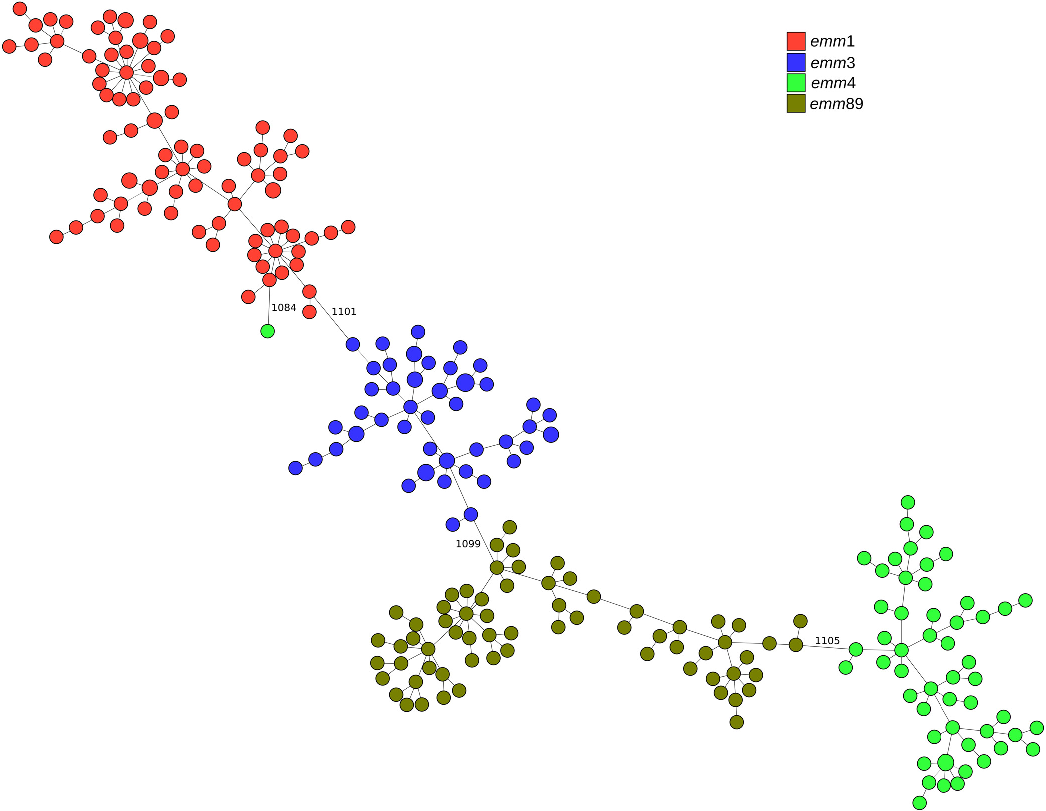
\includegraphics[width=\textwidth]{figures/chapter 4/Figure1.pdf}
    \caption[Minimum-spanning tree generated with the goeBURST algorithm for the cgMLST-100 profiles of 265 \textit{S. pyogenes} isolates recovered in Portugal.]{Minimum-spanning tree generated with the goeBURST algorithm for the cgMLST-100 profiles of 265 \textit{S. pyogenes} isolates recovered in Portugal (see Data Set 1 in \cite{friaes_supplemental_2023}). The size of each node is proportional to the number of isolates with that particular cgMLST-100 profile on a logarithmic scale. Nodes are colored according to \textit{emm} type. Link distances of $\geq1,000$ allelic differences are labeled (from a total of 1,230 compared loci).}
    \label{fig:chap4_figure1}
\end{figure*}

A lower congruence was obtained between the distributions of isolates in the \ac{MST} and the remaining typing methods (\ac{ST}, \ac{PFGE}, SAg profiling, and T type) (Fig. \ref{fig:chap4_figureS3} to \ref{fig:chap4_figureS6}). The \ac{AW} and \ac{AR} values between T types and \ac{MST} groups linked by up to 1,000 different loci were only slightly lower than those of \textit{emm} types (Tables \ref{tab:ch4_tableS3} and \ref{tab:ch4_tableS4}), but T type had a lower typeability since 17 isolates were nontypeable. Although \ac{MST} groups linked by up to 45 different loci resulted in a number of partitions and \ac{SID}s comparable to those of \ac{ST}, SAg profiling, and \ac{PFGE} (Table \ref{tab:ch4_table1}), the \ac{AW} coefficient between \ac{MST} groups linked by up to 45 different loci and these typing methods was lower than that between \ac{MST} groups linked by up to 1,000 different loci and \textit{emm} type (Table \ref{tab:ch4_tableS4}). This means that \ac{MST} groups linked by up to 45 different loci could not confidently predict the \ac{ST}, \ac{PFGE} cluster, or SAg profile, or the converse, which was also reflected in lower \ac{AR} values (<0.900) (Table \ref{tab:ch4_tableS3}).

The use of a \ac{wgMLST} schema instead of a universally defined cgMLST-100 set of loci allows scalable analysis in which higher resolution can be obtained by including larger numbers of common loci when analyzing closely related isolates. As an example, the cgMLST-100 obtained exclusively for the \textit{emm}4 isolates grouped into the same \ac{MST} group linked by up to 1,000 different loci (\textit{n} = 54) comprises 52 profiles of 1,382 cgMLST-100 loci. The \textit{emm}4 isolates presenting the M phenotype of macrolide resistance (erythromycin resistant and clindamycin susceptible) shared ST39 and an SAg profile with most susceptible isolates (see Data Set 1 in \cite{friaes_supplemental_2023}), rendering these two methods unable to differentiate macrolide-resistant isolates. One \ac{PFGE} cluster was associated with macrolide resistance \cite{silva-costa_differences_2012}, although it also included two susceptible isolates. Similarly, one of the \ac{MST} groups linked by up to 33 different loci comprised exclusively all but two of the macrolide-resistant isolates (Fig. \ref{fig:chap4_figureS7}). Not surprisingly, the set of 46 loci that were present universally and exclusively in the subset of erythromycin-resistant isolates (list available in the supplemental material in reference \cite{friaes_supplemental_2023}) represents mostly phage-related genes, including \textit{mef}(A) and \textit{msr}(D), the genes most commonly associated with the M phenotype in \ac{GAS} \cite{silva-costa_macrolide-resistant_2015, iannelli_type_2018}.

\textbf{Performance of the wgMLST schema on a large and genetically diverse data set}. The genetic structure of the \ac{GAS} population is known to vary temporally and geographically, with an associated impact on the disease spectrum and incidence \cite{steer_global_2009, barnett_fall_2018}. To evaluate the performance of the proposed \ac{wgMLST} schema on the analysis of genetically diverse data sets, we used a large collection of isolates previously selected to represent the genetic, geographic, temporal, and clinical diversity of \ac{GAS} \cite{davies_atlas_2019}. A total of 2,006 assemblies were included in the data set, comprising 140 \textit{emm} types and 443 \ac{ST}s and organized into 292 phylogroups defined by \ac{PopPUNK} \cite{davies_atlas_2019, lees_fast_2019} (see Data Set 2 in \cite{friaes_supplemental_2023}).

We defined 1,321-locus cgMLST-95, 1,204-locus cgMLST-99, and 763-locus cgMLST- 100 schemas (available in the supplemental material in \cite{friaes_supplemental_2023}).

Allele call results identified 1,700 cgMLST-100 profiles. The resulting \ac{MST} indicates that many \textit{emm} types include diverse genetic lineages, with 12 of the 19 most prevalent \textit{emm} types (>30 isolates) comprising isolates distributed in multiple tree regions (Fig. \ref{fig:chap4_figure2}). Accordingly, 50 of the 67 \textit{emm} types comprising $\geq10$ isolates included assemblies that differed in >50\% of the 763 cgMLST-100 loci (up to 708 differences [93\%] in \textit{emm}4) (Fig. \ref{fig:chap4_figure3}A). In 31 of these \textit{emm} types, the mean intra-\textit{emm} allelic difference was larger than the smaller difference from another \textit{emm} type (Table \ref{fig:chap4_figureS5}). This is possibly due to the diversity of geographic and temporal origins of the isolates in this data set and is in line with a previous report of genetic heterogeneity within \textit{emm} types \cite{davies_atlas_2019}. It is also reflected in a low congruence between \textit{emm} types and \ac{MST} groups linked by up to 450 different loci despite similar \ac{SID} values (Tables \ref{tab:ch4_tableS6} to \ref{tab:ch4_tableS8}).

The overall congruence between \ac{ST}s and \ac{MST} groups linked by up to 50 different loci was poor although slightly higher than that observed for the less diverse Data Set 1 (\ac{AR} coefficients of 0.810 and 0.709, respectively) (Table \ref{tab:ch4_tableS7}). In contrast, there was good congruence, with high \ac{AW} and \ac{AR} values, between \ac{PopPUNK} phylogroups and \ac{MST} groups linked by up to 200 different loci (Tables \ref{tab:ch4_tableS7} and \ref{tab:ch4_tableS8}). Still, \ac{PopPUNK} phylogroups can be rather diverse, including multiple \ac{ST}s and isolates differing in up to 61\% of the core 763 loci (phylogroup 27) (Fig. \ref{fig:chap4_figure3}B; Table S9 \cite{friaes_supplemental_2023}), highlighting the advantage of using multiple methods for analyzing the evolution of \ac{GAS} lineages.

\textbf{Performance of the wgMLST schema in an outbreak context}. To evaluate the potential contribution of the proposed \ac{wgMLST} schema for outbreak recognition, we used a previously published data set comprising isolates from 21 outbreaks in England and contemporaneous nonrelated isolates with the same \textit{emm} types \cite{coelho_genomic_2019}. A total of 119 outbreak isolates and 170 sporadic isolates were included (see Data Set 3 in \cite{friaes_supplemental_2023}). Allele calling for the 119 outbreak isolates identified 58 profiles of 1,263 cgMLST-100 loci.

\begin{landscape}
%\vspace*{\fill}
\begin{figure*}[!ht]
    \centering
    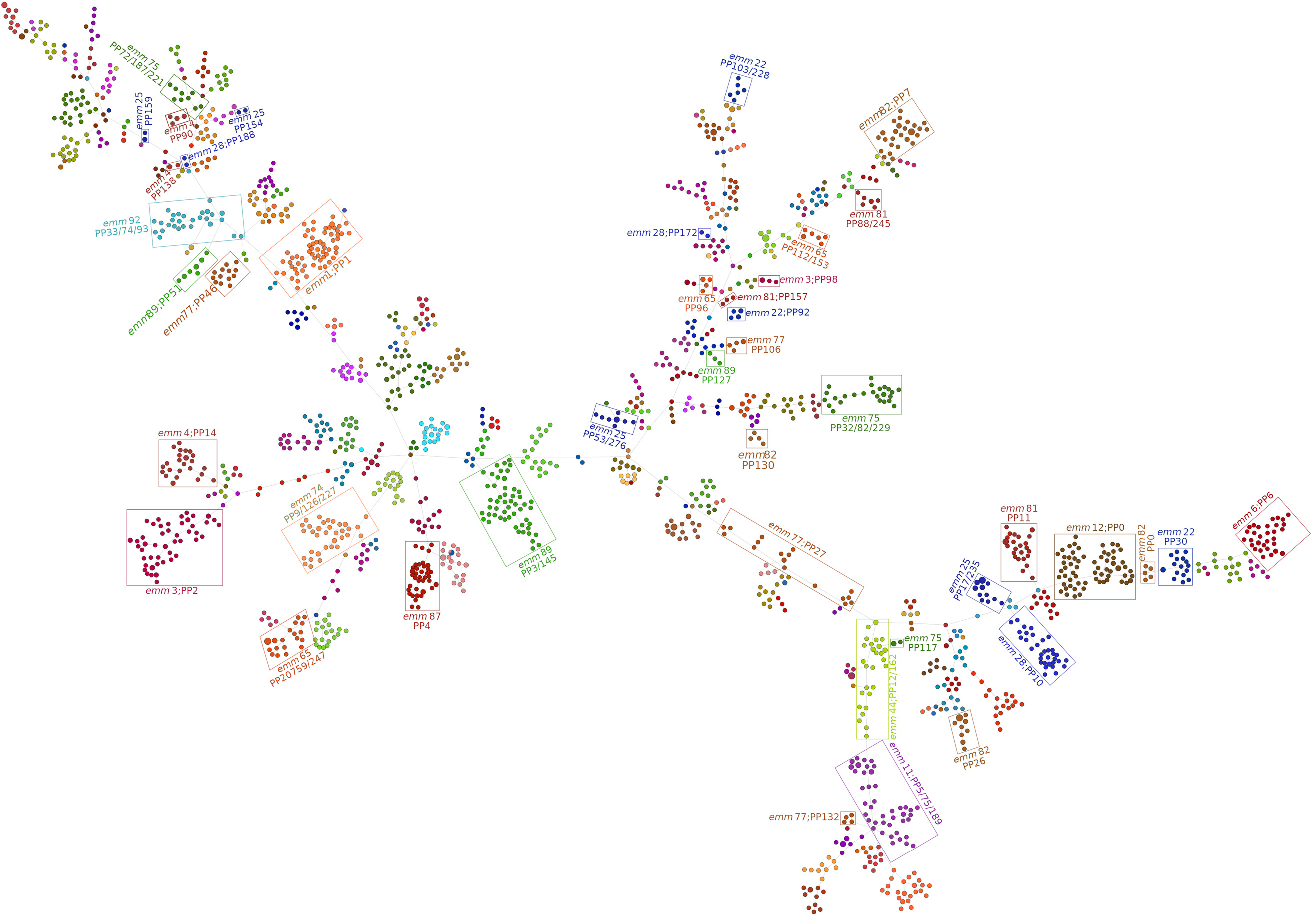
\includegraphics[height=0.85\textheight]{figures/chapter 4/Figure2.pdf}
    \caption[Minimum-spanning tree generated with the goeBURST algorithm for the \ac{cgMLST} profiles of 2,006 genetically diverse \textit{S. pyogenes} isolates recovered worldwide.]{Minimum-spanning tree generated with the goeBURST algorithm for the \ac{cgMLST} profiles of 2,006 genetically diverse \textit{S. pyogenes} isolates recovered worldwide \cite{davies_atlas_2019} (see Data Set 2 in reference \cite{friaes_supplemental_2023}). The size of each node is proportional to the number of isolates with that particular \ac{cgMLST} profile on a logarithmic scale. Nodes are colored according to \textit{emm} type. Groups of clustered \textit{emm} types represented by >30 isolates are highlighted inside rectangles and labeled with the respective \textit{emm} types and PopPUNK phylogroup numbers (for simplicity, isolated nodes of \textit{emm} types 4, 22, 44, 65, 75, 77, 81, and 92 are not highlighted). A total of 763 core loci were compared.}
    \label{fig:chap4_figure2}
\end{figure*}
%\vspace*{\fill}
\end{landscape}

\begin{figure*}[!ht]
    \centering
    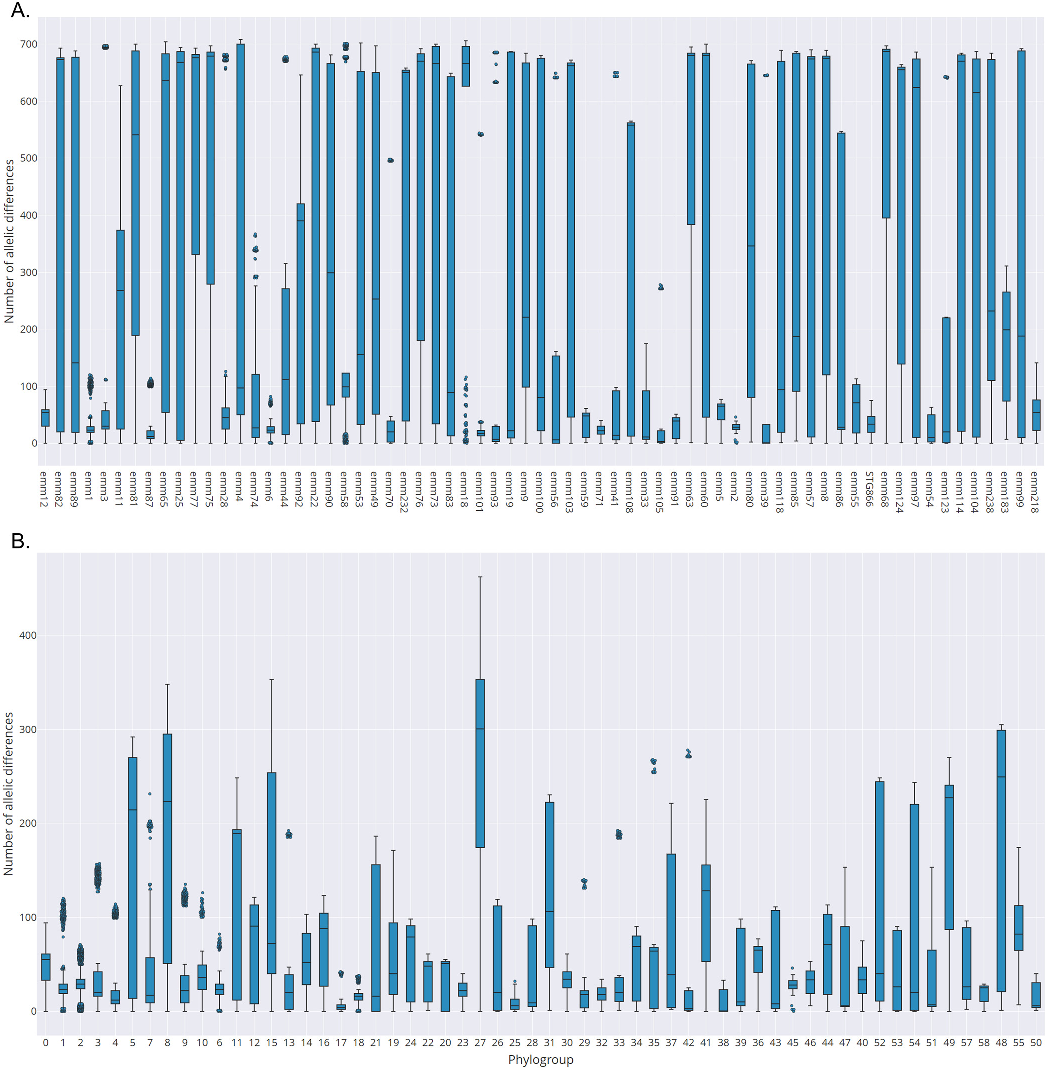
\includegraphics[width=\textwidth]{figures/chapter 4/Figure3.pdf}
    \caption[Box-and-whisker plots for the pairwise distances of the assemblies from Data Set 2 included in each \textit{emm} type with $\geq10$ isolates.]{Box-and-whisker plots for the pairwise distances of the assemblies from Data Set 2 \cite{davies_atlas_2019, friaes_supplemental_2023} included in each \textit{emm} type with $\geq10$ isolates (A) or in each PopPUNK phylogroup with $\geq10$ isolates (B). The distances were calculated based on the allele call results for the 763 cgMLST-100 loci of the 2,006 assemblies (interactive versions of these plots are available as supplemental material in reference \cite{friaes_supplemental_2023}).}
    \label{fig:chap4_figure3}
\end{figure*}

In agreement with the \ac{SNP}-based clustering presented previously \cite{coelho_genomic_2019}, the \ac{MST} clustered the isolates according to \textit{emm} type, with a minimum distance of 1,079 allelic differences between isolates of different \textit{emm} types, while isolates of different subtypes or outbreaks of the same \textit{emm} type were more closely related (Fig. \ref{fig:chap4_figure4}). Individual \ac{MST}s were created for \textit{emm} types 1, 5, 11, 28, 75, 89, and 94, including outbreak and sporadic isolates (Fig. \ref{fig:chap4_figureS8} to \ref{fig:chap4_figureS14}). Since these \ac{MST}s included only isolates sharing the same \textit{emm} type, they comprised larger sets of cgMLST-100 loci (1,384 to 1,547 loci), potentially allowing higher resolution in the discrimination of outbreak isolates. Ten isolates with epidemiological links could be excluded from the respective outbreaks because they did not cluster with isolates of the same outbreak or differed by too many loci (Table \ref{tab:ch4_tableS10} and Fig. \ref{fig:chap4_figureS8} and \ref{fig:chap4_figureS11} to \ref{fig:chap4_figureS13}). These isolates also matched the outbreak exclusion criteria based on \ac{SNP} analysis \cite{coelho_genomic_2019}. Except for these 10 excluded isolates, outbreak isolates linked in the \ac{MST}s shared >99.5\% of their core genome (maximum link distance of 6 allelic differences), and the mean distance within a given outbreak was much lower than the mean distance among sporadic isolates of the same \textit{emm} type (Table \ref{tab:ch4_table2}). However, in \textit{emm} types 1 and 5, there were sporadic isolates with \ac{cgMLST} profiles very similar to those of outbreak 1 (OB1) and OB19, respectively (0 to 2 allelic differences), indicating that these outbreak strains were also present in the community (Table \ref{tab:ch4_table2}; Fig. \ref{fig:chap4_figureS8} and \ref{fig:chap4_figureS9}).

\begin{figure*}[!ht]
    \centering
    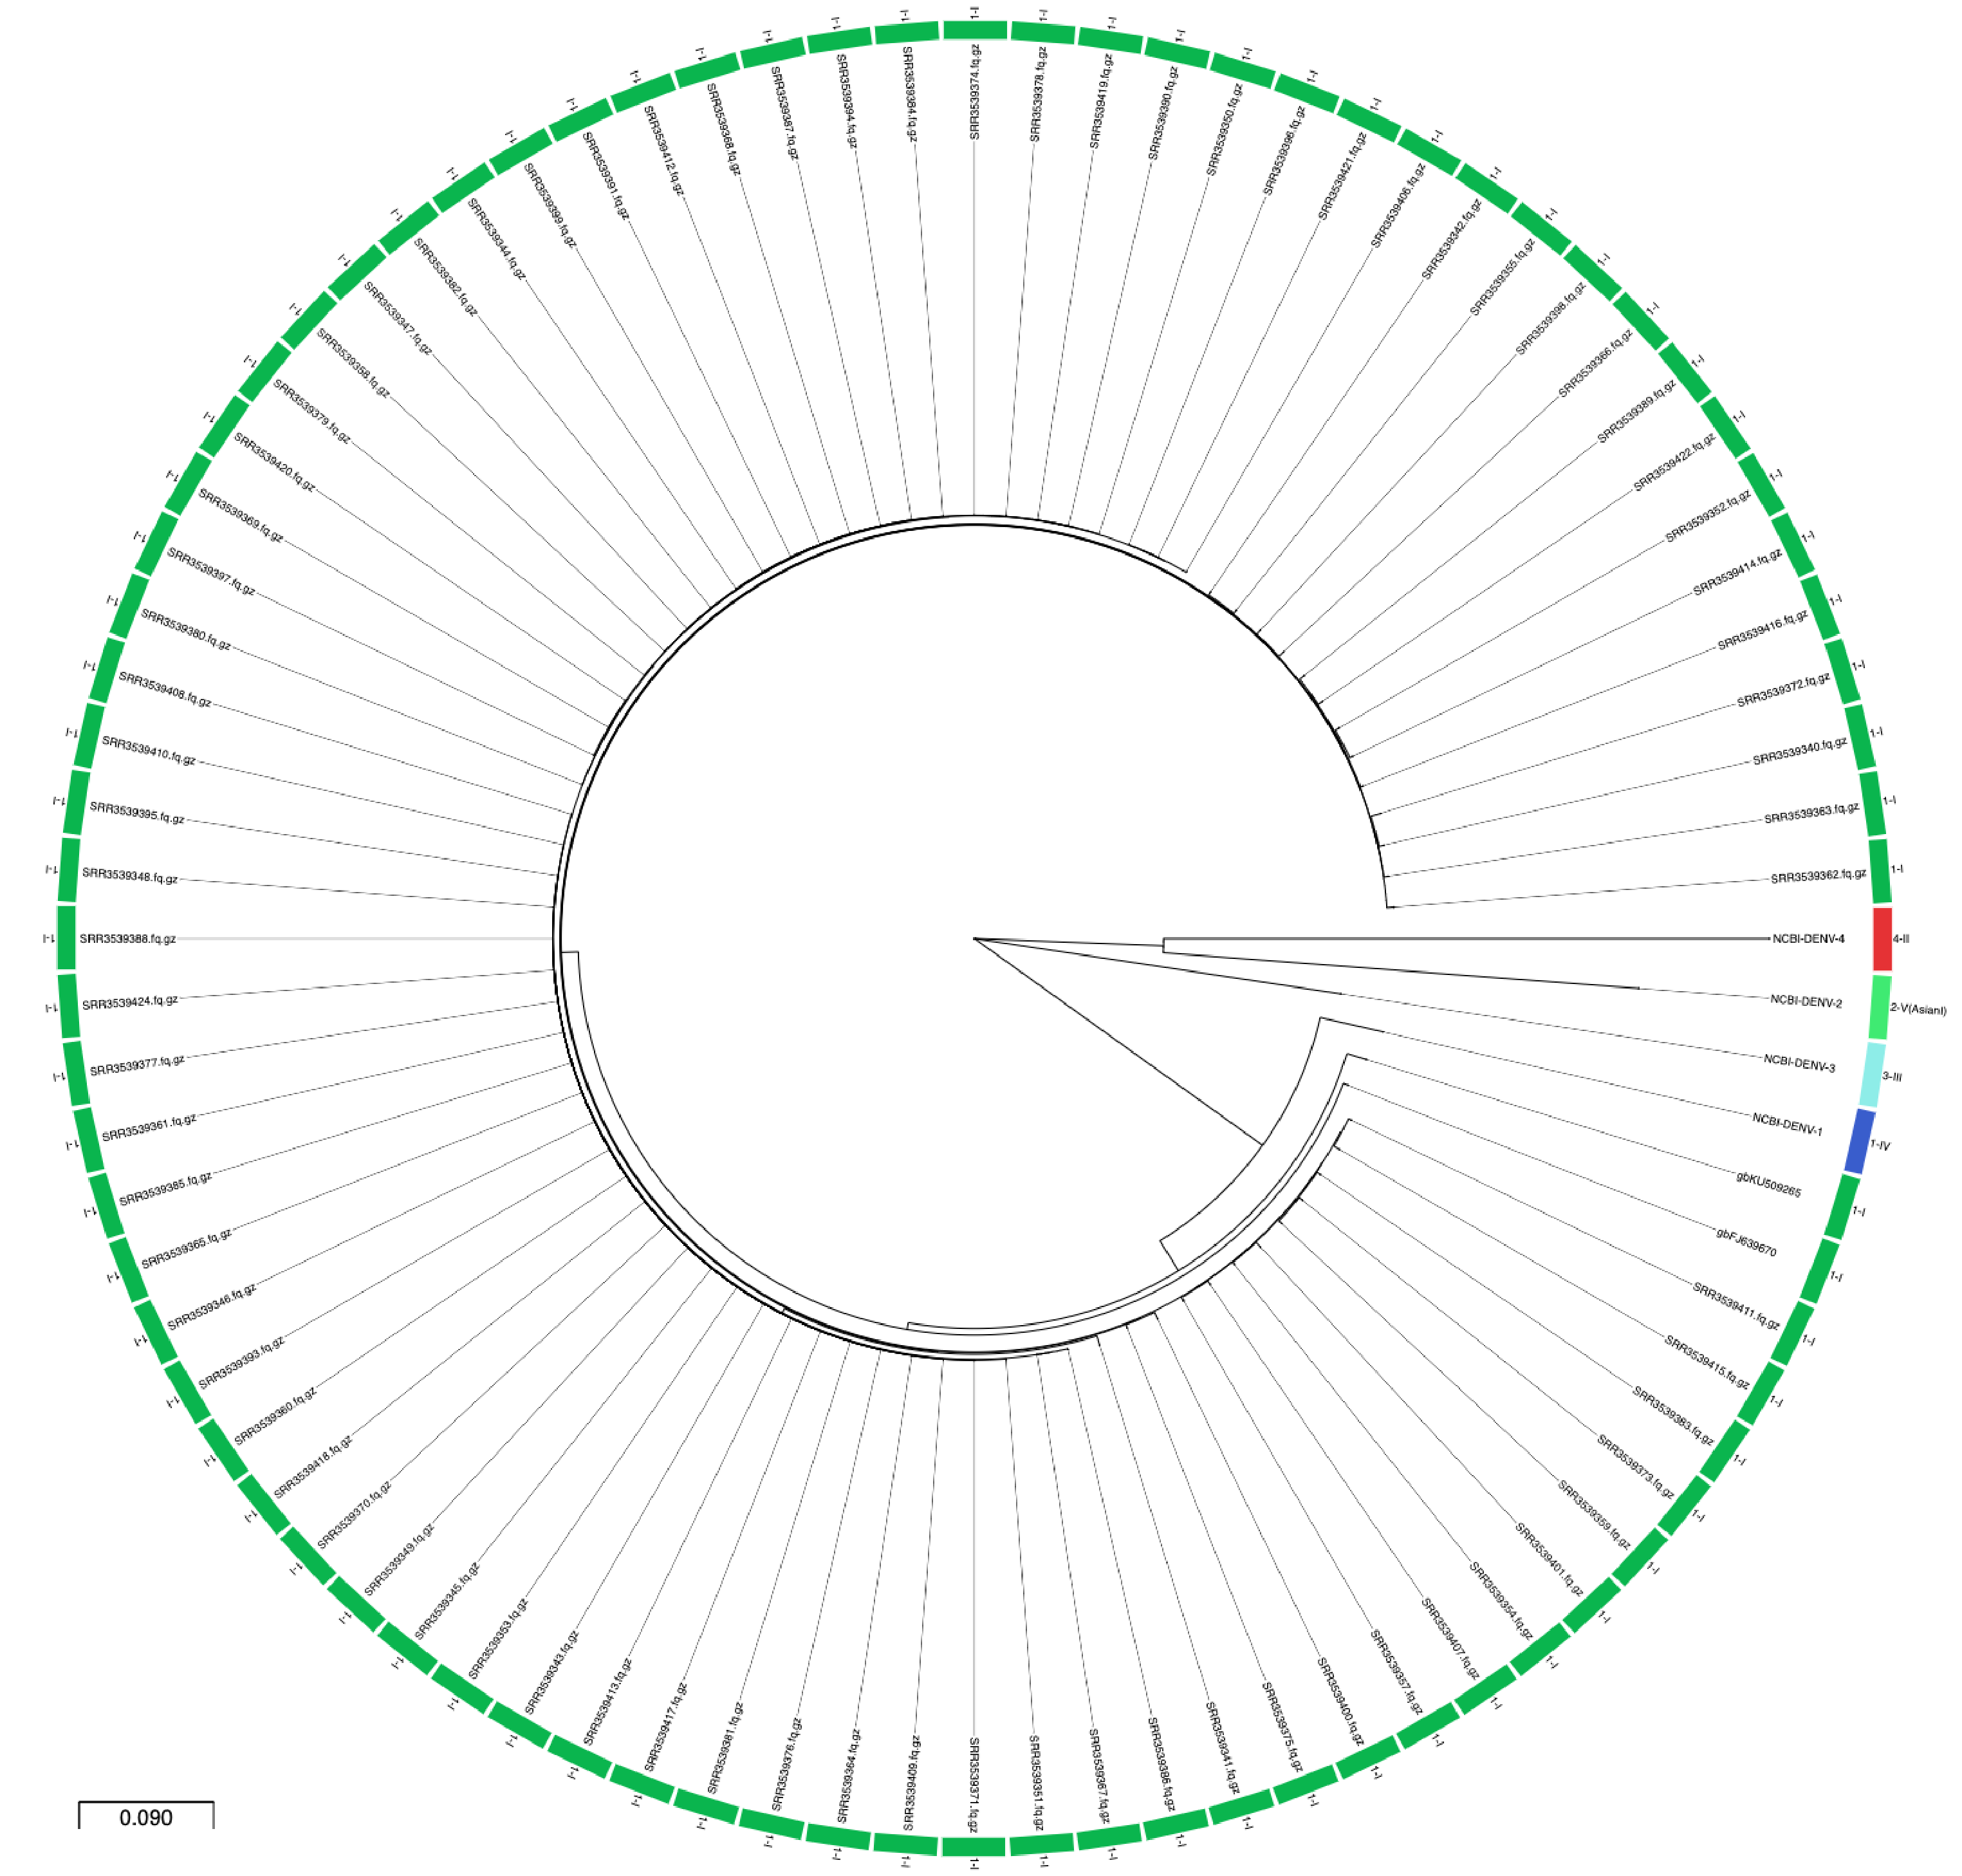
\includegraphics[width=\textwidth]{figures/chapter 4/Figure4.pdf}
    \caption[Minimum-spanning tree generated with the goeBURST algorithm for the cgMLST-100 profiles of 119 outbreak \textit{S. pyogenes} isolates recovered in the United Kingdom.]{Minimum-spanning tree generated with the goeBURST algorithm for the cgMLST-100 profiles of 119 outbreak \textit{S. pyogenes} isolates recovered in the United Kingdom \cite{coelho_genomic_2019} (see Data Set 3 in reference \cite{friaes_supplemental_2023}). The size of each node is proportional to the number of isolates with that particular \ac{cgMLST} profile on a logarithmic scale. The nodes are colored according to the \textit{emm} type, and the outer ring is colored according to the outbreak number. Link distances are labeled as the number of allelic differences between nodes (from a total of 1,263 compared loci).}
    \label{fig:chap4_figure4}
\end{figure*}

\begin{table}[!ht]
    \centering
    \resizebox{\linewidth}{!}{
    \begin{threeparttable}[b]
    \caption[Distances (numbers of allelic differences) among outbreak isolates and between each outbreak and sporadic isolates of the same \textit{emm} type determined by cgMLST-100 analysis for each \textit{emm} type, using a collection of isolates from the United Kingdom.]{Distances (numbers of allelic differences) among outbreak isolates and between each outbreak and sporadic isolates of the same \textit{emm} type determined by cgMLST-100 analysis for each \textit{emm} type, using a collection of isolates from the United Kingdom\tnote{a}}
    \label{tab:ch4_table2}
    \begin{tabular}{@{}lllll@{}}
        \toprule
        \multicolumn{1}{|c|}{\textit{emm} type} & \multicolumn{1}{|c|}{No. loci in cgMLST} & \multicolumn{1}{|c|}{Subset (no. isolates)} & \multicolumn{1}{|c|}{Mean distance within subset (range)} & \multicolumn{1}{|c|}{Mean distance to sporadic isolates (range)} \\ \midrule
        1 & 1488 & OB1 (6) & 0.6 (0-1) & 17.9 (2-59) \\
        ~ & OB3 (6) & 1.7 (1-2) & 18.4 (8-53) & ~ \\
        ~ & OB4 (4) & 0.5 (0-1) & 24.8 (15-60) & ~ \\
        ~ & OB6 (3) & 0.7 (0-1) & 50.1 (46-55) & ~ \\
        ~ & Sporadic (30) & 25.7 (3-63) & NA & ~ \\
        5 & 1485 & OB19 (14) & 1.6 (0-4) & 124.1 (0-174) \\
        ~ & Sporadic (27) & 112.0 (0-175) & NA & ~ \\
        11 & 1384 & OB20 (10) & 3.8 (0-8) & 89.8 (35-592) \\
        ~ & Sporadic (26) & 118.6 (1-597) & NA & ~ \\
        28 & 1510 & OB21 (2) & 0 & 44 (12-67) \\
        ~ & Sporadic (11) & 51.0 (0-74) & NA & ~ \\
        75 & 1547 & OB8 (2) & 0 & 20.1 (14-65) \\
        ~ & OB10 (11) & 5.4 (0-11) & 19.6 (12-70) & ~ \\
        ~ & Sporadic (39) & 19.5 (0-76) & NA & ~ \\
        89 & 1392 & OB13 (17) & 0.93 (0-2) & 28.4 (11-42) \\
        ~ & OB14 (3) & 1.3 (1-2) & 29.0 (16-41) & ~ \\
        ~ & OB15 (3) & 0 (0-0) & 32.5 (16-47) & ~ \\
        ~ & OB16 (4) & 0.5 (0-1) & 33.1 (14-45) & ~ \\
        ~ & Sporadic (31) & 31.7 (0-50) & NA & ~ \\
        94 & 1506 & OB17 (3) & 2.7 (1-4) & 29.6 (10-48) \\
        ~ & Sporadic (6) & 31.4 (2-50) & NA & ~ \\
        \bottomrule
    \end{tabular}
    \begin{tablenotes}
       \item [a] {\footnotesize See reference \cite{coelho_genomic_2019} and Data Set 3 in reference \cite{friaes_supplemental_2023}. Ten outbreak isolates were excluded according to the results of both cgMLST-100 and SNP analyses \cite{coelho_genomic_2019}. NA, not applicable.}
    \end{tablenotes}
    \end{threeparttable}
    }
\end{table}

\textbf{Performance of the wgMLST schema in the identification of recently emerged lineages}. We tested if the proposed \ac{wgMLST} schema has enough discriminatory power to identify two recently emerged intra-\textit{emm} lineages that were originally identified by whole-genome \ac{SNP} analysis, namely, $M1_{UK}$ and \textit{emm}89 clade 3 \cite{turner_emergence_2015, zhu_molecular_2015, lynskey_emergence_2019}. Allele calling was performed for the 135 assemblies from noninvasive \textit{emm}1 isolates \cite{lynskey_emergence_2019} together with the complete genome of strain MGAS5005, a reference representative of the $M1_{global}$ lineage (see Data Set 4 in \cite{friaes_supplemental_2023}). The graph in Fig. \ref{fig:chap4_figure5} represents the resulting \ac{MST} with all links of up to 19 differences depicted. All $M1_{UK}$ isolates were tightly clustered, together with an intermediate isolate ($M1_{inter}$) carrying 23 of the 27 \acp{SNP}s characteristic of the $M1_{UK}$ lineage \cite{lynskey_emergence_2019}. The \ac{MST} links within this cluster ranged between 0 and 13 differences, while the closest links to the $M1_{inter}$ cluster (13 \acp{SNP}) and an $M1_{global}$ isolate were 20 and 31 differences, respectively. $M1_{global}$ isolates presented higher genomic diversity, with \ac{MST} links of up to 49 differences. Allele calling was performed for all \textit{emm}89 assemblies included in the four data sets described above and all the complete \textit{emm}89 genomes used to create the schema (\textit{n} = 201) (see Data Set 5 in \cite{friaes_supplemental_2023}). In addition, the P\textit{nga} variant was determined for all isolates. The absence of the \textit{hasA} gene of the capsule locus was confirmed in all P\textit{nga}-3 isolates, while all other isolates carried this gene, except for two ST568 isolates that have an internal nonsense codon in \textit{hasA}. The graph depicting all links of up to 55 differences (Fig. \ref{fig:chap4_figure6}) showed limited diversity in the isolates carrying P\textit{nga}-3, which clustered closely, with \ac{MST} links with 0 to 27 differences, while the shortest link to a P\textit{nga}-2 isolate was 57 differences. The P\textit{nga}-2 and, especially, P\textit{nga}-1 isolates were more diverse, presenting fewer links with up to 55 differences and comprising multiple sublineages associated with different \ac{ST}s (Fig. \ref{fig:chap4_figure6}; Fig. \ref{fig:chap4_figureS15}). Both the wider geographic range and collection time span may contribute to this higher diversity. As previously reported \cite{friaes_emergence_2015}, \ac{MLST} was not suitable for discriminating P\textit{nga}-3 isolates from those carrying P\textit{nga}-2 since ST101 was prevalent among both lineages (Fig. \ref{fig:chap4_figureS15}). Analysis of the \textit{emm}89 isolates from Data Set 1 showed that P\textit{nga}-3 isolates and most P\textit{nga}-2 isolates were also grouped into the same \ac{PFGE} cluster, and some of them shared the same SAg profile, while the T serotype B3264 was ubiquitous, except for the single P\textit{nga}-1 isolate (T11) and one P\textit{nga}-3 isolate that was nontypeable (Fig. \ref{fig:chap4_figureS16} to \ref{fig:chap4_figureS18}). \ac{PopPUNK} clustering also could not discriminate P\textit{nga}-3 isolates, which were clustered with isolates carrying P\textit{nga}-1 and P\textit{nga}-2 in phylogroup 3 (see Data Set 5 in \cite{friaes_supplemental_2023}).

\section{Discussion} \label{sec:ch4_discussion}

The reduced costs of \ac{HTS} have facilitated a wider application of whole-genome data to the epidemiological surveillance of multiple pathogens. This leads to a requirement for standardized analysis pipelines producing reproducible and portable results that can be easily compared across laboratories and with those of previously used typing methods \cite{sabat_overview_2013}. Here, we propose a \ac{wgMLST} schema for \textit{S. pyogenes}, consisting of 3,044 loci. Hard-desined \ac{cgMLST} schemas comprising the subsets of loci present in 95\% (1,321 loci), 99\% (1,204 loci), and 100\% (763 loci) of the assemblies of a collection representing the genetic diversity of \textit{S. pyogenes} \cite{davies_atlas_2019} are also presented.

\begin{figure*}[!ht]
    \centering
    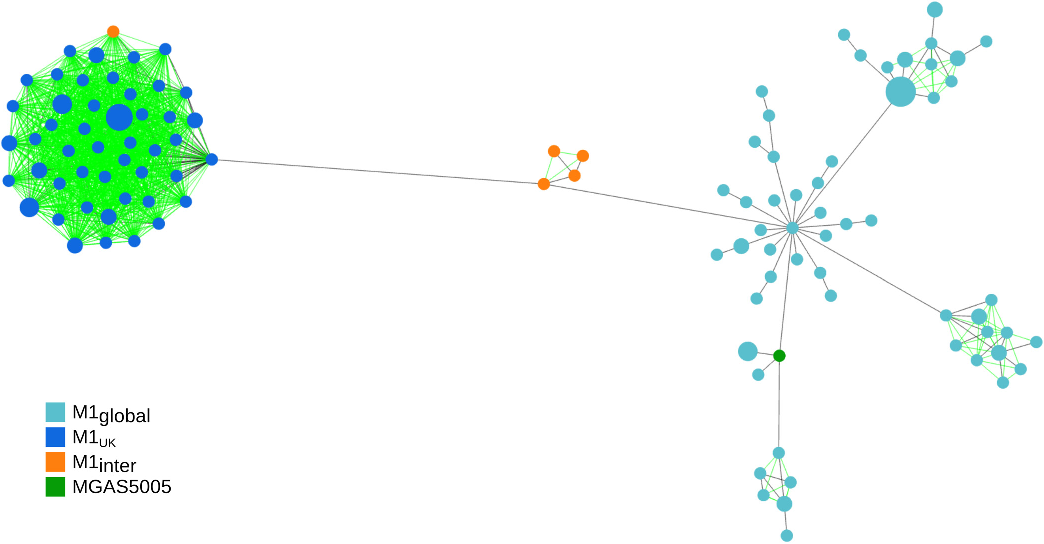
\includegraphics[width=\textwidth]{figures/chapter 4/Figure5.pdf}
    \caption[Graph representation of the relationships between the cgMLST-100 profiles of 135 noninvasive \textit{emm}1 isolates recovered in the United Kingdom and reference strain MGAS5005, depicting all links with $\leq19$ allelic differences (from a total of 1,404 compared loci).]{Graph representation of the relationships between the cgMLST-100 profiles of 135 noninvasive \textit{emm}1 isolates recovered in the United Kingdom \cite{lynskey_emergence_2019} and reference strain MGAS5005 (see Data Set 4 in reference \cite{friaes_supplemental_2023}), depicting all links with $\leq19$ allelic differences (from a total of 1,404 compared loci). The size of each node is proportional to the number of isolates with that particular cgMLST-100 profile on a logarithmic scale. Nodes are colored according to the M1 lineage, with MGAS5005 (reference genome for the $M1_{global}$ lineage) in green. Links that would not be present in the standard \ac{MST} are shown in green. Links shown in black represent the \ac{MST} links and may represent distances with >19 allelic differences.}
    \label{fig:chap4_figure5}
\end{figure*}

However, the use of a \ac{wgMLST} schema from which the \ac{cgMLST} loci are selected according to the specific data set under analysis has the advantage of allowing the inclusion of larger subsets of loci and, hence, increased resolution when comparing closely related isolates \cite{maiden_mlst_2013}. This can be particularly important to track the emergence of intra-\textit{emm}-type sublineages or identify outbreak-related isolates. The application of the schema proposed here to previously published data sets and analysis of the resulting \ac{MST}s showed a performance comparable to that of \ac{SNP}-based methods in distinguishing recently emerged intra-\textit{emm}-type sublineages as well as in identifying clusters of epidemiologically and genetically related isolates associated with local, short-term outbreaks \cite{turner_emergence_2015, lynskey_emergence_2019, coelho_genomic_2019}. Analyses based on \ac{wg/cgMLST} build upon the strengths of \ac{GbG} approaches, which do not require a reference genome or the removal of regions of recombination \cite{maiden_mlst_2013, neumann_core_2019, leopold_bacterial_2014}. This is particularly important when analyzing collections of genetically diverse lineages, such as in long-term surveillance studies, particularly in organisms where mobile genetic elements and recombination play major roles in genomic plasticity and evolution, such as \textit{S. pyogenes} \cite{davies_atlas_2019, mcgregor_multilocus_2004}. Moreover, \ac{GbG} approaches constitute a framework that has been widely used in surveillance, which can facilitate the transition to \ac{wg/cgMLST} by reference laboratories involved in surveillance activities. Comparison of \ac{cgMLST}-based clustering with other typing methods used for \textit{S. pyogenes} revealed poor concordance, although in temporally and geographically restricted data sets, the groups defined by \textit{emm} typing were also supported by \ac{cgMLST}. By including a much higher number of loci, \ac{cgMLST} was expected to present a higher discriminatory power than the traditional seven-gene \ac{MLST} schema and to further discriminate isolates sharing the same \ac{ST} \cite{neumann_core_2019, bletz_defining_2018}. However, such a simplistic expectation was not universally borne out by the data, which highlights the limitations of the seven-gene \ac{MLST} schema to correctly identify \ac{GAS} lineages based on broader genomic information. It is worth noting that from the seven genes included in traditional \ac{MLST}, two (\textit{gtr} and \textit{yqiL}) were excluded from the \ac{wgMLST} schema because they shared alleles with paralogous genes, and one (\textit{xpt}) was absent in at least one \ac{GAS} lineage and therefore was not always included in the \ac{cgMLST} analysis. In contrast, a good correlation was found between \ac{cgMLST} clustering and \ac{PopPUNK} \cite{davies_atlas_2019, lees_fast_2019}, another whole-genome-based clustering method. However, the flexibility of \ac{wg/cgMLST} allows increased resolution by lowering the number of allelic differences used to define clusters and a dynamic \ac{cgMLST} definition, providing further discrimination within \ac{PopPUNK} clusters. The proposed \ac{wgMLST} schema is publicly available on the \ac{Chewie-NS} platform \cite{mamede_chewie_2021}, where multiple statistics regarding the whole schema and individual loci can be visualized (\url{https://chewbbaca.online/species/1/schemas/1}).

\begin{figure*}[!ht]
    \centering
    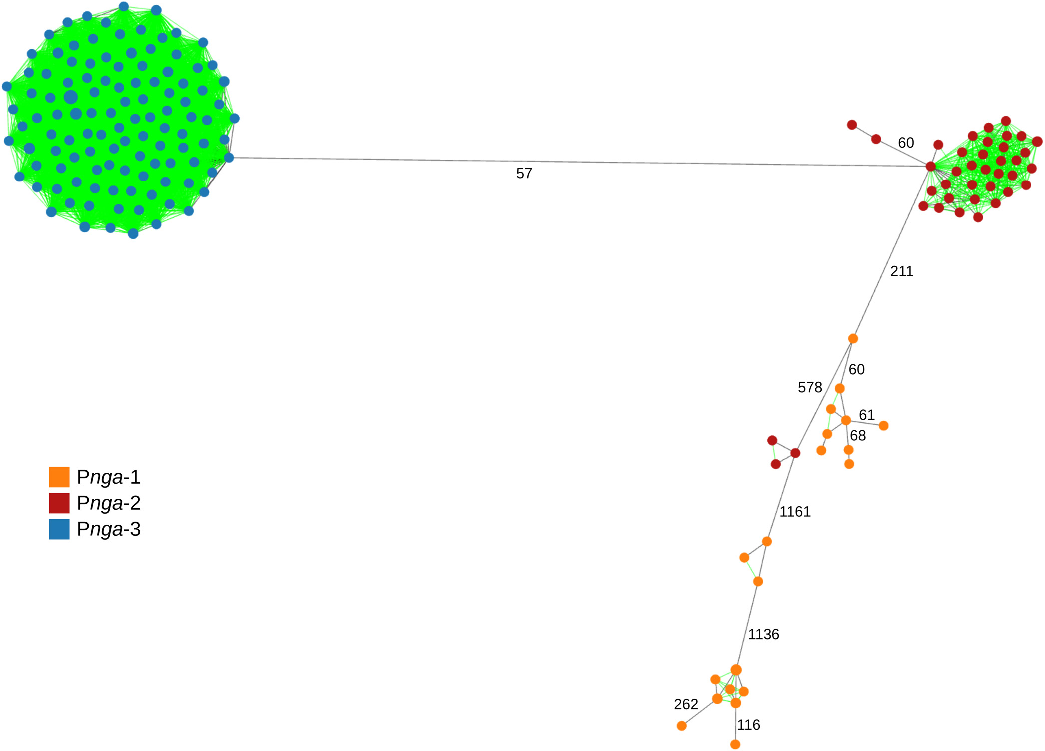
\includegraphics[width=\textwidth]{figures/chapter 4/Figure6.pdf}
    \caption[Graph representation of the relationships between the cgMLST-100 profiles of 201 \textit{emm}89 isolates, depicting all links with $\leq55$ allelic differences (from a total of 1,279 compared loci).]{Graph representation of the relationships between the cgMLST-100 profiles of 201 \textit{emm}89 isolates (see Data Set 5 in reference \cite{friaes_supplemental_2023}) depicting all links with $\leq55$ allelic differences (from a total of 1,279 compared loci). The size of each node is proportional to the number of isolates with that particular cgMLST-100 profile on a logarithmic scale. Nodes are colored according to the variant of the \textit{nga} promoter (P\textit{nga}). Links that would not be present in the standard \ac{MST} are shown in green. Links shown in black represent the \ac{MST} links and may represent distances with >55 allelic differences (labeled links).}
    \label{fig:chap4_figure6}
\end{figure*}

The close integration with the chewBBACA suite \cite{silva_chewbbaca_2018} facilitates its use in surveillance and epidemiological studies and the maintenance of a common nomenclature across different studies. By virtue of the comprehensive annotation, the database can be used to obtain relevant data for basic research, such as the variability of genes of interest (virulence factors, antimicrobial resistance genes, candidate vaccine antigens, and transcriptional regulators, etc.) \cite{davies_atlas_2019, beres_integrative_2022} in addition to its use for typing purposes.

\section{Acknowledgments} \label{sec:ch4_acknowledgments}

R.M. was supported by the \ac{FCT} (grant 2020.08493.BD). Partial support was received from the ONEIDA project (LISBOA-01-0145-FEDER-016417), cofunded by the FEEI (Fundos Europeus Estruturais e de Investimento) from the Programa Operacional Regional de Lisboa, Portugal, 2020 (POR Lisboa 2020), and by national funds from the \ac{FCT} and the LISBOA-01-0145-FEDER-007391 project, cofunded by FEDER through POR Lisboa 2020 and the \ac{FCT}.

\newpage

\section{Supplemental Material} \label{sec:ch4_supplemental_material}

\subsection{Supplemental Figures} \label{ssec:ch4_supplemental_figures}

\begin{figure*}[!ht]
    \centering
    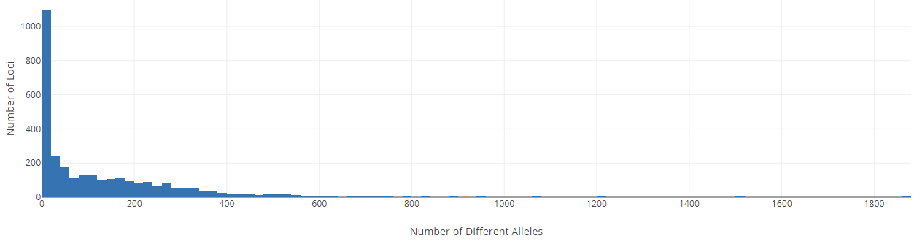
\includegraphics[angle=0,width=\textwidth]{figures/chapter 4/FigureS1.pdf}
    \caption[Number of loci with given number of alleles in the wgMLST schema of \textit{S. pyogenes}.]{Number of loci with given number of alleles in the \ac{wgMLST} schema of \textit{S. pyogenes} (\url{https://chewbbaca.online/species/1/schemas/1}).}
    \label{fig:chap4_figureS1}
\end{figure*}

\begin{figure*}[!ht]
    \centering
    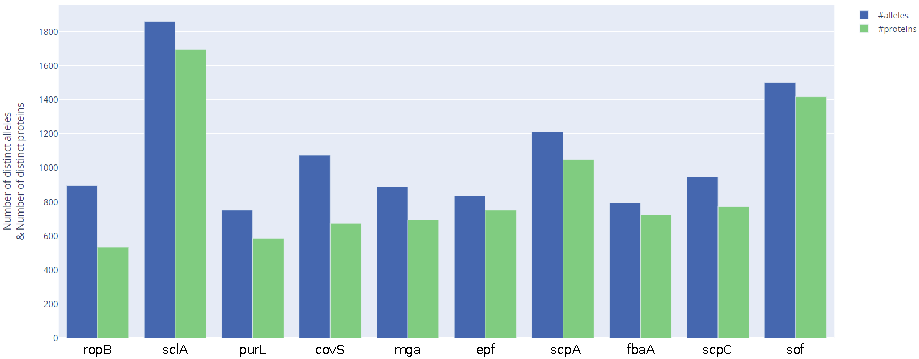
\includegraphics[angle=0,width=\textwidth]{figures/chapter 4/FigureS2.pdf}
    \caption[Number of DNA alleles and protein variants of the 10 loci with the largest number of distinct alleles in the \textit{S. pyogenes} wgMLST schema.]{Number of \ac{DNA} alleles and protein variants of the 10 loci with the largest number of distinct alleles in the \textit{S. pyogenes} \ac{wgMLST} schema.}
    \label{fig:chap4_figureS2}
\end{figure*}

\newpage
\begin{figure*}[!ht]
    \centering
    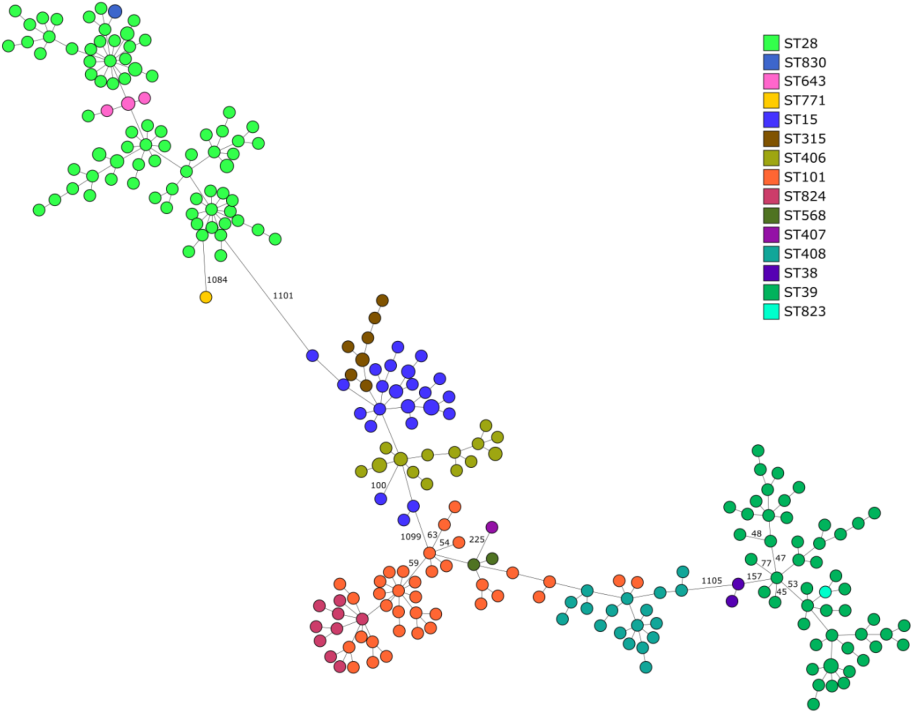
\includegraphics[angle=0,width=\textwidth]{figures/chapter 4/FigureS3.pdf}
    \caption[Minimum spanning tree generated with the goeBURST algorithm for the cgMLST profiles of 265 \textit{S. pyogenes} isolates recovered in Portugal.]{Minimum spanning tree generated with the goeBURST algorithm for the \ac{cgMLST} profiles of 265 \textit{S. pyogenes} isolates recovered in Portugal [Dataset 1 \cite{friaes_supplemental_2023}]. Nodes are colored according to \ac{ST}. The size of each node is proportional to the number of isolates with that particular \ac{cgMLST} profile on a logarithmic scale. Link distances $\geq45$ differences are labeled (from a total of 1,230 compared loci).}
    \label{fig:chap4_figureS3}
\end{figure*}

\newpage
\begin{figure*}[!ht]
    \centering
    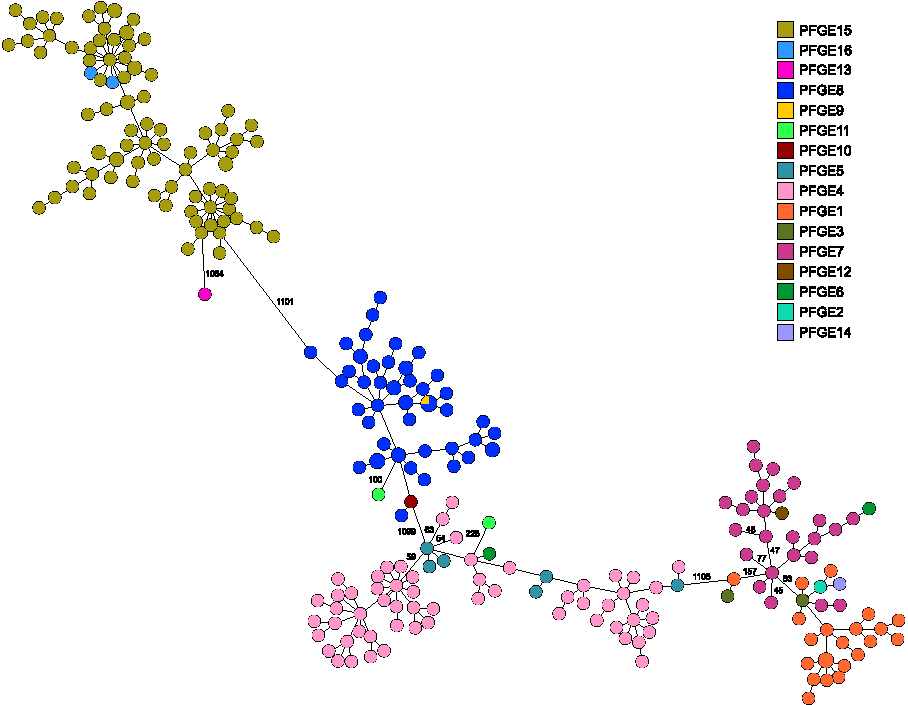
\includegraphics[angle=0,width=\textwidth]{figures/chapter 4/FigureS4.pdf}
    \caption[Minimum spanning tree generated with the goeBURST algorithm for the cgMLST profiles of 265 \textit{S. pyogenes} isolates recovered in Portugal.]{Minimum spanning tree generated with the goeBURST algorithm for the \ac{cgMLST} profiles of 265 \textit{S. pyogenes} isolates recovered in Portugal [Dataset 1 \cite{friaes_supplemental_2023}]. Nodes are colored according to \ac{PFGE} cluster. The size of each node is proportional to the number of isolates with that particular \ac{cgMLST} profile on a logarithmic scale. Link distances $\geq45$ differences are labeled (from a total of 1,230 compared loci).}
    \label{fig:chap4_figureS4}
\end{figure*}

\newpage
\begin{figure*}[!ht]
    \centering
    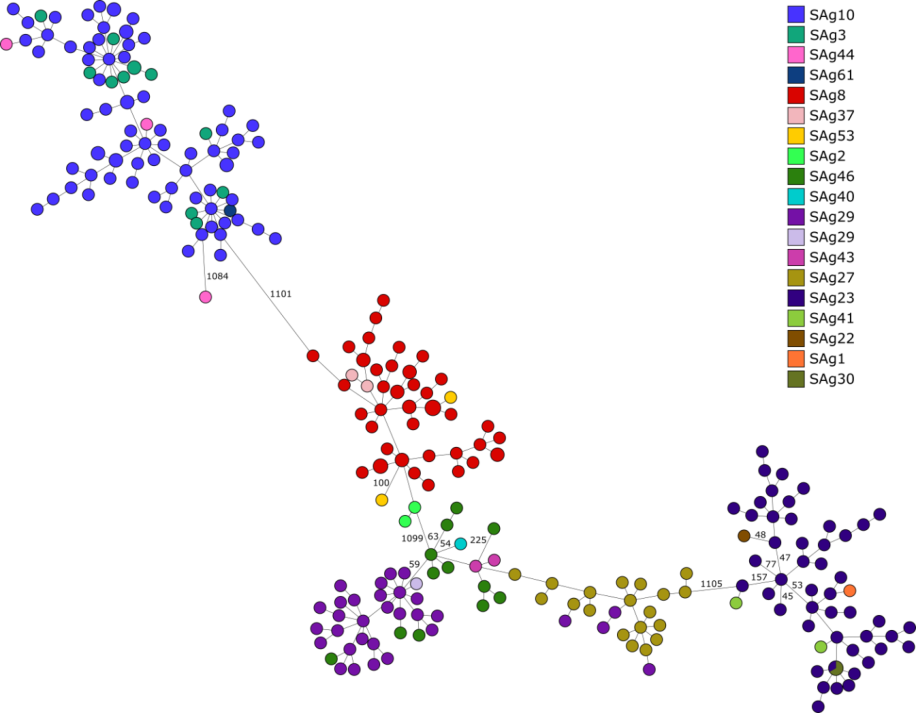
\includegraphics[angle=0,width=\textwidth]{figures/chapter 4/FigureS5.pdf}
    \caption[Minimum spanning tree generated with the goeBURST algorithm for the cgMLST profiles of 265 \textit{S. pyogenes} isolates recovered in Portugal.]{Minimum spanning tree generated with the goeBURST algorithm for the \ac{cgMLST} profiles of 265 \textit{S. pyogenes} isolates recovered in Portugal [Dataset 1 \cite{friaes_supplemental_2023}]. Nodes are colored according to SAg profile. The size of each node is proportional to the number of isolates with that particular \ac{cgMLST} profile on a logarithmic scale. Link distances $\geq45$ differences are labeled (from a total of 1,230 compared loci).}
    \label{fig:chap4_figureS5}
\end{figure*}

\newpage
\begin{figure*}[!ht]
    \centering
    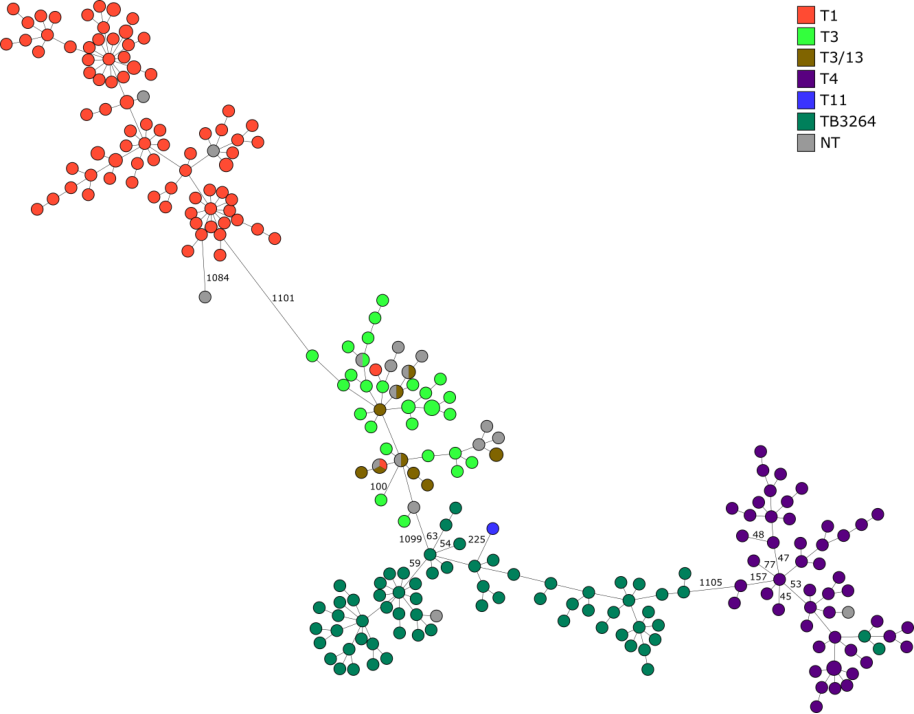
\includegraphics[angle=0,width=\textwidth]{figures/chapter 4/FigureS6.pdf}
    \caption[Minimum spanning tree generated with the goeBURST algorithm for the cgMLST profiles of 265 \textit{S. pyogenes} isolates recovered in Portugal.]{Minimum spanning tree generated with the goeBURST algorithm for the \ac{cgMLST} profiles of 265 \textit{S. pyogenes} isolates recovered in Portugal [Dataset 1 \cite{friaes_supplemental_2023}]. Nodes are colored according to T-type. The size of each node is proportional to the number of isolates with that particular \ac{cgMLST} profile on a logarithmic scale. Link distances $\geq45$ differences are labeled (from a total of 1,230 compared loci). NT, non-typeable.}
    \label{fig:chap4_figureS6}
\end{figure*}

\newpage
\begin{figure*}[!ht]
    \centering
    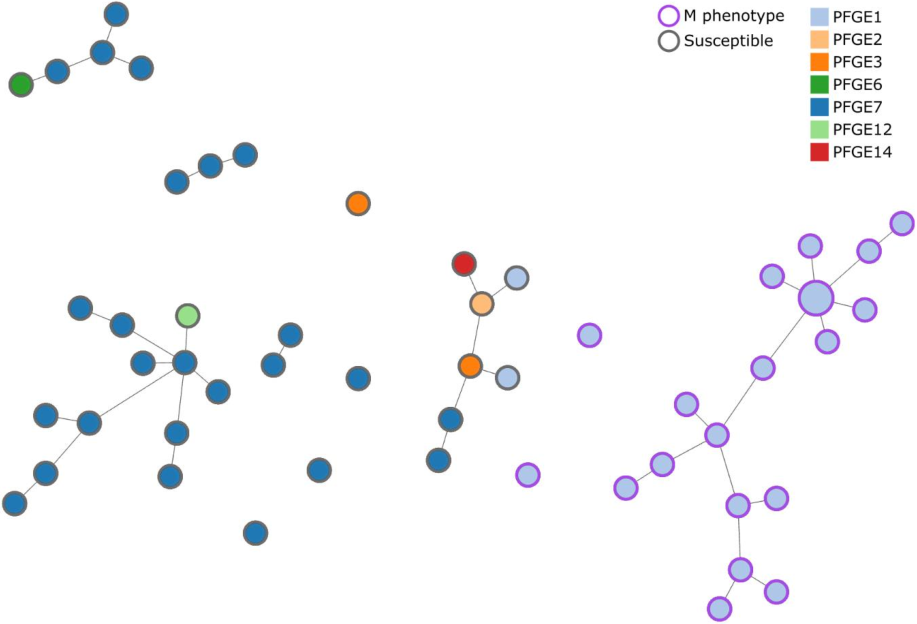
\includegraphics[angle=0,width=\textwidth]{figures/chapter 4/FigureS7.pdf}
    \caption[Representation of the MST groups defined at 33 allelic differences cutoff (from a total of 1,382 compared loci) for 54 \textit{emm}4 isolates recovered in Portugal.]{Representation of the \ac{MST} groups defined at 33 allelic differences cutoff (from a total of 1,382 compared loci) for 54 \textit{emm}4 isolates recovered in Portugal [Dataset 1 \cite{friaes_supplemental_2023}]. The nodes are colored according to \ac{PFGE} cluster and the outer ring according to macrolide resistance phenotype. The size of each node is proportional to the number of isolates with that particular \ac{cgMLST} profile on a logarithmic scale. M phenotype, erythromycin-resistant and clindamycin-susceptible.}
    \label{fig:chap4_figureS7}
\end{figure*}

\newpage
\begin{figure*}[!ht]
    \centering
    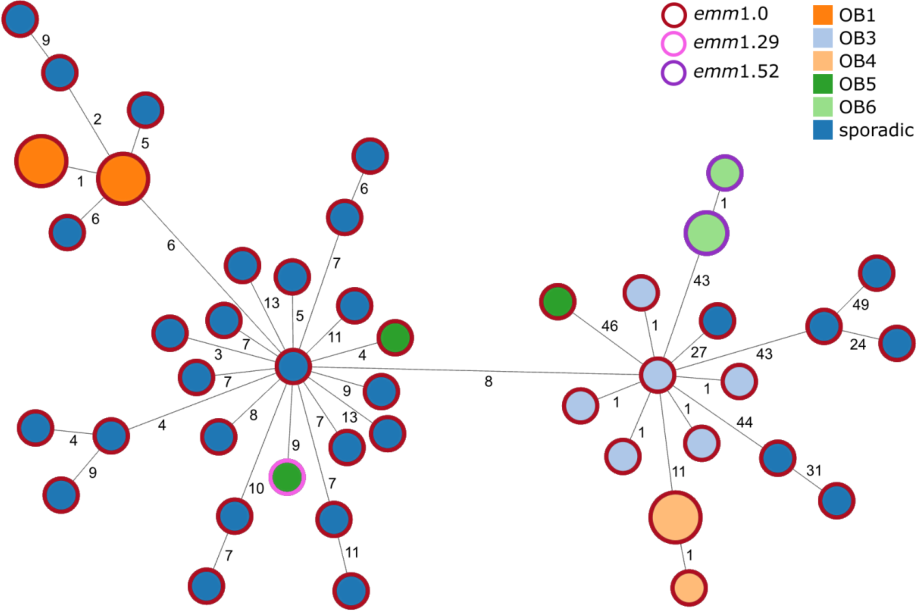
\includegraphics[angle=0,width=\textwidth]{figures/chapter 4/FigureS8.pdf}
    \caption[Minimum spanning tree generated with the goeBURST algorithm for the cgMLST profiles of 22 outbreak and 30 sporadic \textit{emm}1 isolates recovered in the UK.]{Minimum spanning tree generated with the goeBURST algorithm for the \ac{cgMLST} profiles of 22 outbreak and 30 sporadic \textit{emm}1 isolates recovered in the UK \cite{coelho_genomic_2019} [Dataset 3 \cite{friaes_supplemental_2023}]. The size of each node is proportional to the number of isolates with that particular \ac{cgMLST} profile on a logarithmic scale. The nodes are colored according to outbreak number and the outer ring according to \textit{emm} subtype. Outbreak 2 was not included because after assembly and the exclusion criteria were applied only one representative isolate was kept, which was excluded from the outbreak by \ac{SNP} analysis \cite{coelho_genomic_2019}. Link distances are represented as the total number of allelic differences between nodes (from a total of 1,488 compared loci). All isolates belong to \ac{ST}28.}
    \label{fig:chap4_figureS8}
\end{figure*}

\newpage
\begin{figure*}[!ht]
    \centering
    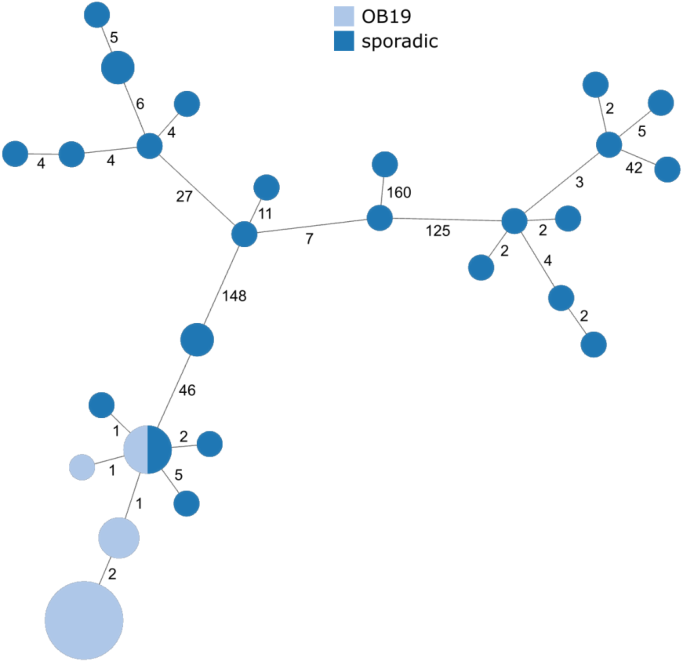
\includegraphics[angle=0,width=\textwidth]{figures/chapter 4/FigureS9.pdf}
    \caption[Minimum spanning tree generated with the goeBURST algorithm for the cgMLST profiles of 14 outbreak and 27 sporadic \textit{emm}5 isolates recovered in the UK.]{Minimum spanning tree generated with the goeBURST algorithm for the \ac{cgMLST} profiles of 14 outbreak and 27 sporadic \textit{emm}5 isolates recovered in the UK \cite{coelho_genomic_2019} [Dataset 3 \cite{friaes_supplemental_2023}]. The size of each node is proportional to the number of isolates with that particular \ac{cgMLST} profile on a logarithmic scale. Nodes are colored according to outbreak number. Link distances are represented as the total number of allelic differences between nodes (from a total of 1,485 compared loci). All isolates belong to \ac{ST}99.}
    \label{fig:chap4_figureS9}
\end{figure*}

\newpage
\begin{figure*}[!ht]
    \centering
    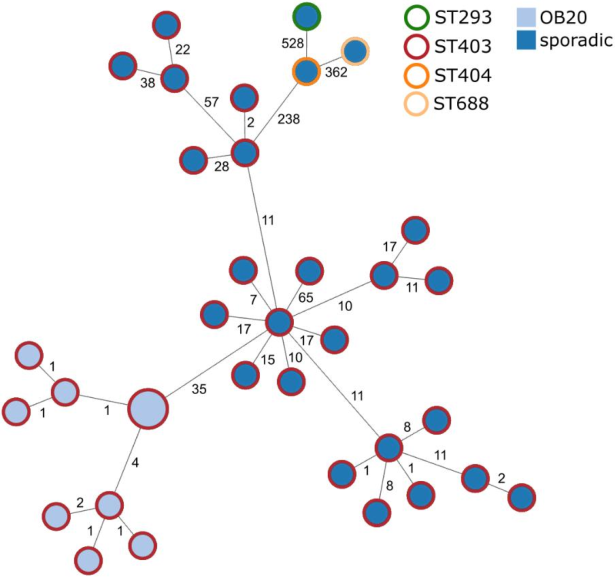
\includegraphics[angle=0,width=\textwidth]{figures/chapter 4/FigureS10.pdf}
    \caption[Minimum spanning tree generated with the goeBURST algorithm for the cgMLST profiles of 10 outbreak and 26 sporadic \textit{emm}11 isolates recovered in the UK.]{Minimum spanning tree generated with the goeBURST algorithm for the \ac{cgMLST} profiles of 10 outbreak and 26 sporadic \textit{emm}11 isolates recovered in the UK \cite{coelho_genomic_2019} [Dataset 3 \cite{friaes_supplemental_2023}]. The size of each node is proportional to the number of isolates with that particular \ac{cgMLST} profile on a logarithmic scale. The nodes are colored according to outbreak number and the outer ring according to \ac{ST}. Link distances are represented as the total number of allelic differences between nodes (from a total of 1,384 compared loci).}
    \label{fig:chap4_figureS10}
\end{figure*}

\newpage
\begin{figure*}[!ht]
    \centering
    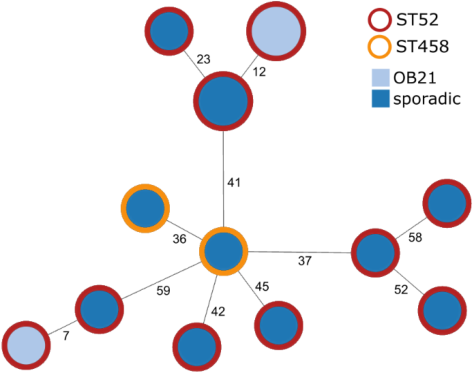
\includegraphics[angle=0,width=\textwidth]{figures/chapter 4/FigureS11.pdf}
    \caption[Minimum spanning tree generated with the goeBURST algorithm for the cgMLST profiles of 3 outbreak and 11 sporadic \textit{emm}28 isolates recovered in the UK.]{Minimum spanning tree generated with the goeBURST algorithm for the \ac{cgMLST} profiles of 3 outbreak and 11 sporadic \textit{emm}28 isolates recovered in the UK \cite{coelho_genomic_2019} [Dataset 3 \cite{friaes_supplemental_2023}]. The size of each node is proportional to the number of isolates with that particular \ac{cgMLST} profile on a logarithmic scale. The nodes are colored according to outbreak number and the outer ring according to \ac{ST}. Link distances are represented as the total number of allelic differences between nodes (from a total of 1,510 compared loci).}
    \label{fig:chap4_figureS11}
\end{figure*}

\newpage
\begin{figure*}[!ht]
    \centering
    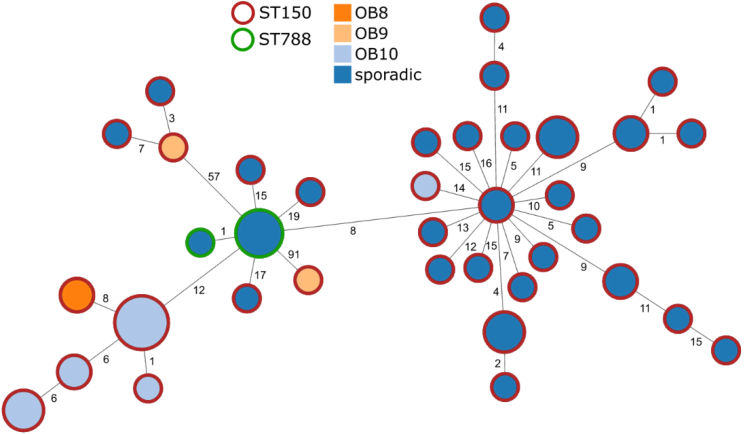
\includegraphics[angle=0,width=\textwidth]{figures/chapter 4/FigureS12.pdf}
    \caption[Minimum spanning tree generated with the goeBURST algorithm for the cgMLST profiles of 16 outbreak and 39 sporadic \textit{emm}75 isolates recovered in the UK.]{Minimum spanning tree generated with the goeBURST algorithm for the \ac{cgMLST} profiles of 16 outbreak and 39 sporadic \textit{emm}75 isolates recovered in the UK \cite{coelho_genomic_2019} [Dataset 3 \cite{friaes_supplemental_2023}]. The size of each node is proportional to the number of isolates with that particular \ac{cgMLST} profile on a logarithmic scale. The nodes are colored according to outbreak number and the outer ring according to \ac{ST}. Link distances are represented as the total number of allelic differences between nodes (from a total of 1,547 compared loci).}
    \label{fig:chap4_figureS12}
\end{figure*}

\newpage
\begin{figure*}[!ht]
    \centering
    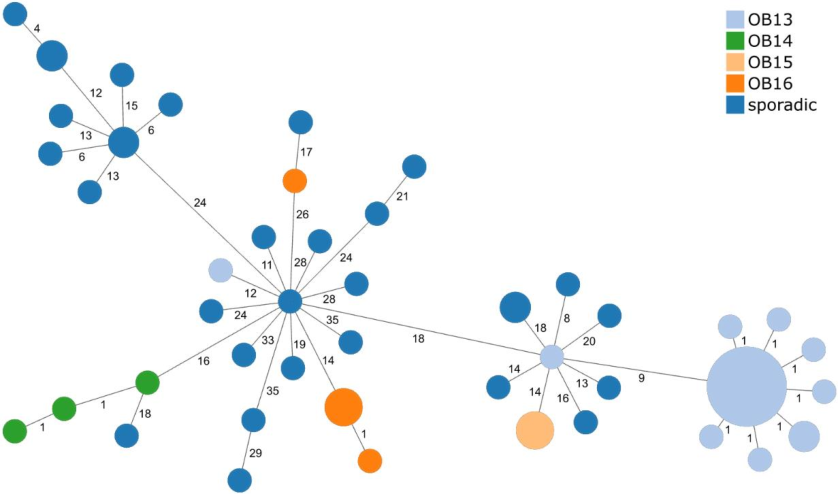
\includegraphics[angle=0,width=\textwidth]{figures/chapter 4/FigureS13.pdf}
    \caption[Minimum spanning tree generated with the goeBURST algorithm for the cgMLST profiles of 30 outbreak and 31 sporadic \textit{emm}89 isolates recovered in the UK.]{Minimum spanning tree generated with the goeBURST algorithm for the \ac{cgMLST} profiles of 30 outbreak and 31 sporadic \textit{emm}89 isolates recovered in the UK \cite{coelho_genomic_2019} [Dataset 3 \cite{friaes_supplemental_2023}]. The size of each node is proportional to the number of isolates with that particular \ac{cgMLST} profile on a logarithmic scale. Nodes are colored according to outbreak number. Link distances are represented as the total number of allelic differences between nodes (from a total of 1,392 compared loci). All isolates belong to \ac{ST}101.}
    \label{fig:chap4_figureS13}
\end{figure*}

\newpage
\begin{figure*}[!ht]
    \centering
    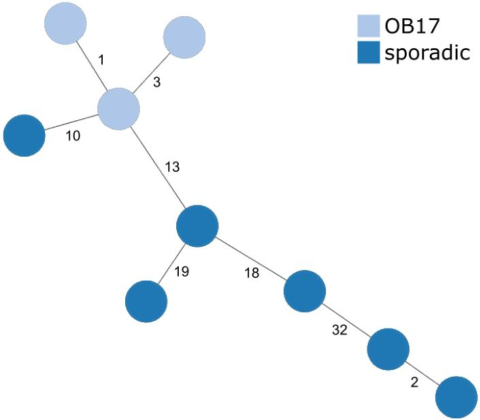
\includegraphics[angle=0,width=\textwidth]{figures/chapter 4/FigureS14.pdf}
    \caption[Minimum spanning tree generated with the goeBURST algorithm for the cgMLST profiles of 3 outbreak and 6 sporadic \textit{emm}94 isolates recovered in the UK.]{Minimum spanning tree generated with the goeBURST algorithm for the \ac{cgMLST} profiles of 3 outbreak and 6 sporadic \textit{emm}94 isolates recovered in the UK \cite{coelho_genomic_2019} [Dataset 3 \cite{friaes_supplemental_2023}]. The size of each node is proportional to the number of isolates with that particular \ac{cgMLST} profile on a logarithmic scale. Nodes are colored according to outbreak number. Link distances are represented as the total number of allelic differences between nodes (from a total of 1,506 compared loci). All isolates belong to \ac{ST}89.}
    \label{fig:chap4_figureS14}
\end{figure*}

\newpage
\begin{figure*}[!ht]
    \centering
    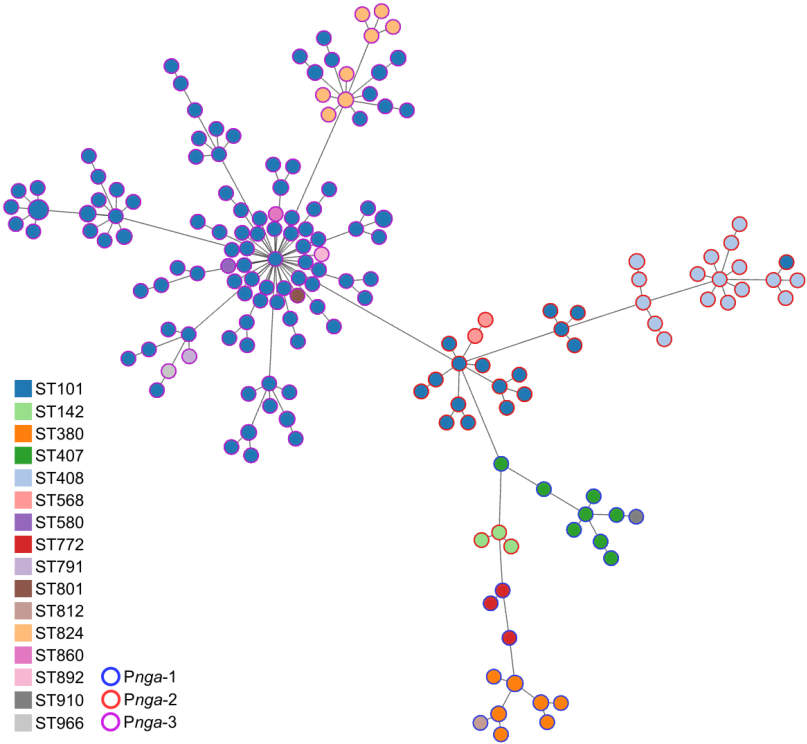
\includegraphics[angle=0,width=\textwidth]{figures/chapter 4/FigureS15.pdf}
    \caption[Minimum spanning tree generated with the goeBURST algorithm for the cgMLST profiles of 201 \textit{emm}89 isolates.]{Minimum spanning tree generated with the goeBURST algorithm for the \ac{cgMLST} profiles of 201 \textit{emm}89 isolates [Dataset 5 \cite{friaes_supplemental_2023}]. The size of each node is proportional to the number of isolates with that particular \ac{cgMLST} profile on a logarithmic scale. The nodes are colored according to ST and the outer ring according to the variant of the \textit{nga} promoter (P\textit{nga}). A total of 1,279 loci were compared.}
    \label{fig:chap4_figureS15}
\end{figure*}

\newpage
\begin{figure*}[!ht]
    \centering
    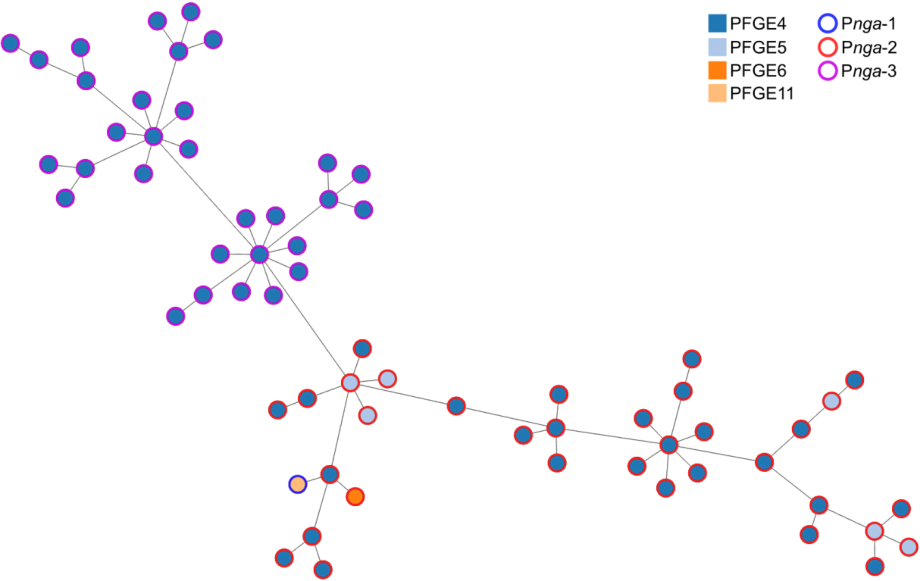
\includegraphics[angle=0,width=\textwidth]{figures/chapter 4/FigureS16.pdf}
    \caption[Minimum spanning tree generated with the goeBURST algorithm for the cgMLST profiles of 66 \textit{emm}89 isolated in Portugal.]{Minimum spanning tree generated with the goeBURST algorithm for the \ac{cgMLST} profiles of 66 \textit{emm}89 isolated in Portugal [Dataset 1 and Dataset 5 \cite{friaes_supplemental_2023}]. The size of each node is proportional to the number of isolates with that particular \ac{cgMLST} profile on a logarithmic scale. The nodes are colored according to \ac{PFGE} cluster and the outer ring according to the variant of the \textit{nga} promoter (P\textit{nga}). A total of 1,388 loci were compared.}
    \label{fig:chap4_figureS16}
\end{figure*}

\newpage
\begin{figure*}[!ht]
    \centering
    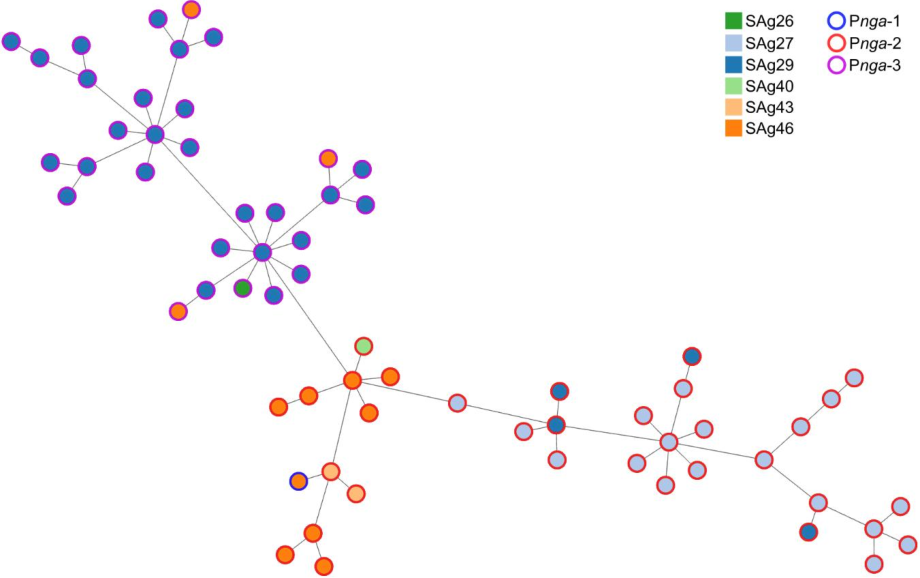
\includegraphics[angle=0,width=\textwidth]{figures/chapter 4/FigureS17.pdf}
    \caption[Minimum spanning tree generated with the goeBURST algorithm for the cgMLST profiles of 66 \textit{emm}89 isolated in Portugal.]{Minimum spanning tree generated with the goeBURST algorithm for the \ac{cgMLST} profiles of 66 \textit{emm}89 isolated in Portugal [Dataset 1 and Dataset 5 \cite{friaes_supplemental_2023}]. The size of each node is proportional to the number of isolates with that particular \ac{cgMLST} profile on a logarithmic scale. The nodes are colored according to SAg gene profile and the outer ring according to the variant of the \textit{nga} promoter (P\textit{nga}). A total of 1,388 loci were compared.}
    \label{fig:chap4_figureS17}
\end{figure*}

\newpage
\begin{figure*}[!ht]
    \centering
    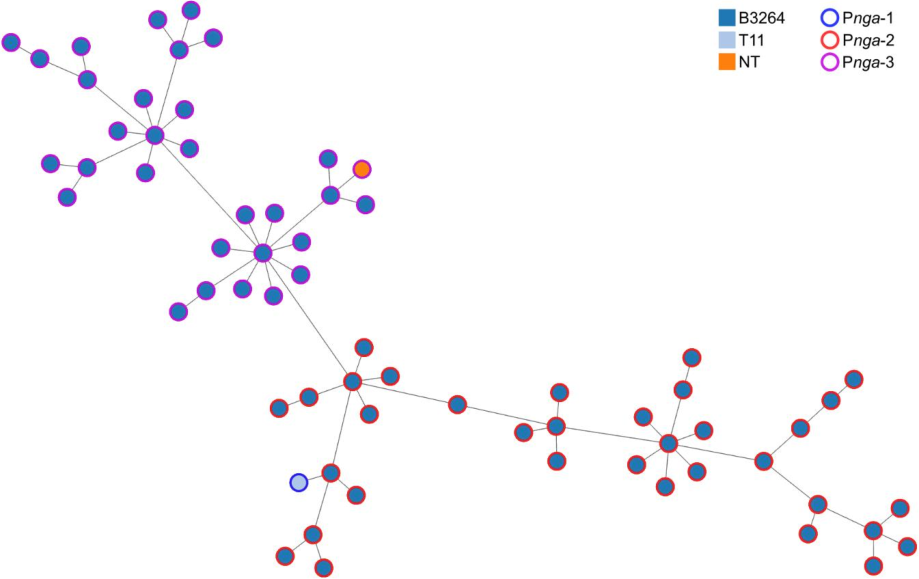
\includegraphics[angle=0,width=\textwidth]{figures/chapter 4/FigureS18.pdf}
    \caption[Minimum spanning tree generated with the goeBURST algorithm for the cgMLST profiles of 66 \textit{emm}89 isolated in Portugal.]{Minimum spanning tree generated with the goeBURST algorithm for the \ac{cgMLST} profiles of 66 \textit{emm}89 isolated in Portugal [Dataset 1 and Dataset 5 \cite{friaes_supplemental_2023}]. The size of each node is proportional to the number of isolates with that particular \ac{cgMLST} profile on a logarithmic scale. The nodes are colored according to T-type and the outer ring according to the variant of the \textit{nga} promoter (P\textit{nga}). A total of 1,388 loci were compared.}
    \label{fig:chap4_figureS18}
\end{figure*}

\newpage

\subsection{Supplemental Tables} \label{ssec:ch4_supplemental_tables}

\noindent \textbf{Table S1} – Complete genomes used for schema creation. See separate \textit{xlsx} file \cite{friaes_supplemental_2023}.

\noindent \textbf{Table S2} – Changes applied to the initial schema. See separate \textit{xlsx} file \cite{friaes_supplemental_2023}.

\newpage
\begin{table}[!ht]
    \centering
    \resizebox{0.95\linewidth}{!}{
    \begin{threeparttable}[b]
    \caption[Adjusted Rand (AR) values for the clustering methods used in the analysis of 265 \textit{S. pyogenes} isolates recovered in Portugal.]{Adjusted Rand (\ac{AR}) values for the clustering methods used in the analysis of 265 \textit{S. pyogenes} isolates recovered in Portugal [Dataset 1 \cite{friaes_supplemental_2023}].}
    \label{tab:ch4_tableS3}
    \begin{tabular}{@{}lllllll@{}}
        \toprule
        \multicolumn{1}{|c|}{} & \multicolumn{1}{|c|}{SAg profile} & \multicolumn{1}{|c|}{\textit{emm} type} & \multicolumn{1}{|c|}{ST} & \multicolumn{1}{|c|}{PFGE} & \multicolumn{1}{|c|}{T-type\tnote{a}} & \multicolumn{1}{|c|}{$MST_{1000}$\tnote{b}} \\ \midrule
        \textit{emm} type & 0.725 & ~ & ~ & ~ & ~ & ~ \\
        ST & 0.65 & 0.755 & ~ & ~ & ~ & ~ \\
        PFGE & 0.705 & 0.861 & 0.675 & ~ & ~ & ~ \\
        T-type\tnote{a} & 0.649 & 0.927 & 0.755 & 0.806 & ~ & ~ \\
        $MST_{1000}$\tnote{b} & 0.729 & 0.996 & 0.759 & 0.865 & 0.927 & ~ \\
        $MST_{45}$\tnote{b} & 0.729 & 0.815 & 0.709 & 0.846 & 0.744 & 0.818 \\
        \bottomrule
    \end{tabular}
    \begin{tablenotes}
       \item [a] {\footnotesize The \ac{AR} values for T-type were calculated for the subset of 248 isolates with a defined T-type (17 isolates were non-typeable).}
       \item [b] {\footnotesize Groups of isolates linked by up to \textit{n} different loci in the MST (MST\textit{n}).}
    \end{tablenotes}
    \end{threeparttable}
    }
\end{table}


\newpage
\begin{landscape}
\vspace*{\fill}
    \begin{table}[!ht]
    \centering
    \resizebox{0.95\linewidth}{!}{
    \begin{threeparttable}[b]
    \caption[Adjusted Wallace (AW) values (95\% confidence intervals) for the clustering methods used in the analysis of 265 \textit{S. pyogenes} isolates recovered in Portugal.]{Adjusted Wallace (\ac{AW}) values (95\% confidence intervals) for the clustering methods used in the analysis of 265 \textit{S. pyogenes} isolates recovered in Portugal [Dataset 1 \cite{friaes_supplemental_2023}].}
    \label{tab:ch4_tableS4}
    \begin{tabular}{@{}lllllllll@{}}
        \toprule
        \multicolumn{1}{|c|}{} & \multicolumn{1}{|c|}{cgMLST-100} & \multicolumn{1}{|c|}{SAg profile} & \multicolumn{1}{|c|}{T-type\tnote{a}} & \multicolumn{1}{|c|}{\textit{emm} type} & \multicolumn{1}{|c|}{ST} & \multicolumn{1}{|c|}{PFGE} & \multicolumn{1}{|c|}{$MST_{1000}$\tnote{b}} & \multicolumn{1}{|c|}{$MST_{45}$\tnote{b}} \\ \midrule
        cgMLST-100 & & \Centerstack{0.904 \\ (0.814-0.995)} & \Centerstack{0.929 \\ (0.858-1.000)} & \Centerstack{1.000 \\ (1.000-1.000)} & \Centerstack{1.000 \\ (1.000-1.000)} & \Centerstack{0.848 \\ (0.688-1.000)} & \Centerstack{1.000 \\ (1.000-1.000)} & \Centerstack{1.000 \\ (1.000-1.000)} \\
        SAg profile & \Centerstack{0.003 \\ (0.000-0.008)} & & \Centerstack{0.885 \\ (0.844-0.927)} & \Centerstack{1.000 \\ (0.999-1.000)} & \Centerstack{0.671 \\ (0.599-0.743)} & \Centerstack{0.821 \\ (0.791-0.851)} & \Centerstack{1.000 \\ (0.999-1.000)} & \Centerstack{0.804 \\ (0.777-0.831)} \\
        T-type\tnote{a} & \Centerstack{0.002 \\ (0.000-0.005)} & \Centerstack{0.512 \\ (0.430-0.594)} & & \Centerstack{0.948 \\ (0.897-0.998)} & \Centerstack{0.627 \\ (0.553-0.702)} & \Centerstack{0.721 \\ (0.648-0.794)} & \Centerstack{0.948 \\ (0.897-0.998)} & \Centerstack{0.632 \\ (0.586-0.679)} \\
        \textit{emm} type & \Centerstack{0.002 \\ (0.000-0.005)} & \Centerstack{0.569 \\ (0.493-0.644)} & \Centerstack{0.907 \\ (0.870-0.945)} & & \Centerstack{0.606 \\ (0.542-0.670)} & \Centerstack{0.756 \\ (0.698-0.815)} & \Centerstack{0.992 \\ (0.977-1.000)} & \Centerstack{0.687 \\ (0.658-0.716)} \\
        ST & \Centerstack{0.003 \\ (0.000-0.008)} & \Centerstack{0.630 \\ (0.539-0.721)} & \Centerstack{0.948 \\ (0.915-0.980)} & \Centerstack{1.000 \\ (1.000-1.000)} & & \Centerstack{0.759 \\ (0.703-0.816)} & \Centerstack{1.000 \\ (1.000-1.000)} & \Centerstack{0.756 \\ (0.725-0.787)} \\
        PFGE & \Centerstack{0.002 \\ (0.000-0.006)} & \Centerstack{0.617 \\ (0.535-0.699)} & \Centerstack{0.915 \\ (0.889-0.942)} & \Centerstack{1.000 \\ (0.999-1.000)} & \Centerstack{0.608 \\ (0.541-0.675)} & & \Centerstack{1.000 \\ (0.999-1.000)} & \Centerstack{0.807 \\ (0.787-0.828)} \\
        $MST_{1000}$ & \Centerstack{0.002 \\ (0.000-0.005)} & \Centerstack{0.573 \\ (0.498-0.648}) & \Centerstack{0.907 \\ (0.870-0.945)} & \Centerstack{1.000 \\ (1.000-1.000)} & \Centerstack{0.611 \\ (0.548-0.674)} & \Centerstack{0.763 \\ (0.704-0.821)} & & \Centerstack{0.693 \\ (0.664-0.721)} \\
        $MST_{45}$ & \Centerstack{0.003 \\ (0.000-0.007)} & \Centerstack{0.666 \\ (0.575-0.757)} & \Centerstack{0.903 \\ (0.872-0.935)} & \Centerstack{1.000 \\ (1.000-1.000)} & \Centerstack{0.667 \\ (0.595-0.739)} & \Centerstack{0.889 \\ (0.833-0.945)} & \Centerstack{1.000 \\ (1.000-1.000)} & \\
        \bottomrule
    \end{tabular}
    \begin{tablenotes}
       \item [a] {\footnotesize The \ac{AW} values for T-type were calculated for the subset of 248 isolates with a defined T-type (17 isolates were non-typeable).}
       \item [b] {\footnotesize Groups of isolates linked by up to \textit{n} different loci in the MST (MST\textit{n}).}
    \end{tablenotes}
    \end{threeparttable}
    }
\end{table}

\vspace*{\fill}
\end{landscape}

\newpage
\noindent \textbf{Table S5} – Minimum, maximum and mean distances (number of allelic differences) among isolates of \textit{emm} types comprising $\geq10$ isolates and shortest distances to other \textit{emm} types. See separate \textit{xlsx} file \cite{friaes_supplemental_2023}.

\newpage
\begin{table}[h!]
    \centering
    \resizebox{0.95\linewidth}{!}{
    \begin{threeparttable}[b]
    \caption{Simpson’s index of diversity (\ac{SID}) and 95\% confidence intervals ($CI_{95\%}$) for the clustering methods used in the analysis of 2,006 genetically diverse \textit{S. pyogenes} isolates recovered worldwide [Dataset 2 \cite{friaes_supplemental_2023}].}
    \label{tab:ch4_tableS6}
    \begin{tabular}{@{}lll@{}}
        \toprule
        \multicolumn{1}{|c|}{Clustering method} & \multicolumn{1}{|c|}{No. of partitions} & \multicolumn{1}{|c|}{SID ($CI_{95\%}$)} \\ \midrule
        \textit{emm} type & 140 & 0.985 (0.984-0.986) \\
        ST & 443 & 0.993 (0.992-0.993) \\
        PopPUNK & 292 & 0.989 (0.989-0.990) \\
        $MST_{450}$\tnote{a} & 192 & 0.985 (0.984-0.986) \\
        $MST_{200}$\tnote{a} & 306 & 0.990 (0.989-0.991) \\
        $MST_{50}$\tnote{a} & 474 & 0.992 (0.991-0.993) \\
        cgMLST-100 & 1700 & 1.000 (1.000-1.000) \\
        \bottomrule
    \end{tabular}
    \begin{tablenotes}
       \item [a] {\footnotesize Groups of isolates linked by up to \textit{} different loci in the MST (MST\textit{n})}
    \end{tablenotes}
    \end{threeparttable}
    }
\end{table}


\newpage
\begin{table}[!ht]
    \centering
    \resizebox{0.95\linewidth}{!}{
    \begin{threeparttable}[b]
    \caption[Adjusted Rand (AR) values for the clustering methods used in the analysis of 2,006 genetically diverse \textit{S. pyogenes} isolates recovered worldwide.]{Adjusted Rand (\ac{AR}) values for the clustering methods used in the analysis of 2,006 genetically diverse \textit{S. pyogenes} isolates recovered worldwide [Dataset 2 \cite{friaes_supplemental_2023}].}
    \label{tab:ch4_tableS7}
    \begin{tabular}{@{}llllll@{}}
        \toprule
        \multicolumn{1}{|c|}{} & \multicolumn{1}{|c|}{\textit{emm} type} & \multicolumn{1}{|c|}{ST} & \multicolumn{1}{|c|}{PopPUNK} & \multicolumn{1}{|c|}{$MST_{450}$\tnote{a}} & \multicolumn{1}{|c|}{$MST_{200}$\tnote{a}} \\ \midrule
        ST & 0.624 & ~ & ~ & ~ & ~ \\
        PopPUNK & 0.773 & 0.802 & ~ & ~ & ~ \\
        $MST_{450}$\tnote{a} & 0.694 & 0.65 & 0.823 & ~ & ~ \\
        $MST_{200}$\tnote{a} & 0.755 & 0.818 & 0.963 & 0.808 & ~ \\
        $MST_{50}$\tnote{a} & 0.683 & 0.81 & 0.856 & 0.688 & 0.872 \\
        \bottomrule
    \end{tabular}
    \begin{tablenotes}
       \item [a] {\footnotesize Groups of isolates linked by up to \textit{n} different loci in the MST (MST\textit{n}).}
    \end{tablenotes}
    \end{threeparttable}
    }
\end{table}


\newpage
\begin{landscape}
\vspace*{\fill}
    \begin{table}[h!]
    \centering
    \resizebox{0.95\linewidth}{!}{
    \begin{threeparttable}[b]
    \caption{Adjusted Wallace (\ac{AW}) values (95\% confidence intervals) for the clustering methods used in the analysis of 2,006 genetically diverse \textit{S. pyogenes} isolates recovered worldwide [Dataset 2 \cite{friaes_supplemental_2023}].}
    \label{tab:ch4_tableS8}
    \begin{tabular}{@{}llllllll@{}}
        \toprule
        \multicolumn{1}{|c|}{} & \multicolumn{1}{|c|}{\textit{emm} type} & \multicolumn{1}{|c|}{ST} & \multicolumn{1}{|c|}{PopPUNK} & \multicolumn{1}{|c|}{$MST_{450}$\tnote{a}} & \multicolumn{1}{|c|}{$MST_{200}$\tnote{a}} & \multicolumn{1}{|c|}{$MST_{50}$\tnote{a}} & \multicolumn{1}{|c|}{cgMLST-100} \\ \midrule
        \textit{emm} type & & \Centerstack{0.463 \\ (0.438-0.488)} & \Centerstack{0.657 \\ (0.636-0.679)} & \Centerstack{0.695 \\ (0.674-0.716)} & \Centerstack{0.634 \\ (0.614-0.654)} & \Centerstack{0.521 \\ (0.499-0.542)} & \Centerstack{0.023 \\ (0.018-0.028)} \\
        ST & \Centerstack{0.958 \\ (0.939-0.977)} & & \Centerstack{0.982 \\ (0.974-0.991)} & \Centerstack{0.998 \\ (0.996-1.000)} & \Centerstack{0.984 \\ (0.976-0.992)} & \Centerstack{0.845 \\ (0.821-0.869)} & \Centerstack{0.047 \\ (0.039-0.056)} \\
        PopPUNK & \Centerstack{0.937 \\ (0.922-0.953)} & \Centerstack{0.677 \\ (0.646-0.708)} & & \Centerstack{1.000 \\ (1.000-1.000)} & \Centerstack{0.948 \\ (0.941-0.955)} & \Centerstack{0.749 \\ (0.725-0.773)} & \Centerstack{0.033 \\ (0.026-0.039)} \\
        $MST_{450}$\tnote{a} & \Centerstack{0.694 \\ (0.669-0.718)} & \Centerstack{0.482 \\ (0.452-0.511)} & \Centerstack{0.700 \\ (0.675-0.725)} & & \Centerstack{0.678 \\ (0.653-0.704)} & \Centerstack{0.524 \\ (0.496-0.552)} & \Centerstack{0.023 \\ (0.018-0.028)} \\
        $MST_{200}$\tnote{a} & \Centerstack{0.933 \\ (0.916-0.949)} & \Centerstack{0.7 \\ (0.668-0.732)} & \Centerstack{0.978 \\ (0.972-0.983)} & \Centerstack{1.000 \\ (1.000-1.000)} & & \Centerstack{0.772 \\ (0.748-0.797)} & \Centerstack{0.034 \\ (0.027-0.040)} \\
        $MST_{50}$\tnote{a} & \Centerstack{0.991 \\ (0.983-1.000)} & \Centerstack{0.778 \\ (0.742-0.813)} & \Centerstack{1.000 \\ (1.000-1.000)} & \Centerstack{1.000 \\ (1.000-1.000)} & \Centerstack{1.000 \\ (1.000-1.000)} & & \Centerstack{0.044 \\ (0.036-0.051)} \\
        cgMLST-100 & \Centerstack{0.996 \\ (0.991-1.000)} & \Centerstack{1.000 \\ (1.000-1.000)} & \Centerstack{1.000 \\ (1.000-1.000)} & \Centerstack{1.000 \\ (1.000-1.000)} & \Centerstack{1.000 \\ (1.000-1.000)} & \Centerstack{1.000 \\ (1.000-1.000)} & \\
        \bottomrule
    \end{tabular}
    \begin{tablenotes}
       \item [a] {\footnotesize Groups of isolates linked by up to \textit{n} different loci in the MST (MST\textit{n}).}
    \end{tablenotes}
    \end{threeparttable}
    }
\end{table}

\vspace*{\fill}
\end{landscape}

\newpage
\noindent \textbf{Table S9} – Minimum, maximum and mean distances (number of allelic differences) among isolates of \ac{PopPUNK} phylogroups comprising  $\geq10$ isolates and shortest distances to other phylogroups. See separate \textit{xlsx} file \cite{friaes_supplemental_2023}.

\newpage
\begin{landscape}
\vspace*{\fill}
    \begin{table}[h!]
    \centering
    \resizebox{0.80\linewidth}{!}{
    \begin{threeparttable}[b]
    \caption{Isolates with epidemiological links to outbreak isolates \cite{coelho_genomic_2019} that were excluded based on cgMLST analysis. Distances are expressed as number of allelic differences.}
    \label{tab:ch4_tableS10}
    \begin{tabular}{@{}llllll@{}}
        \toprule
        \multicolumn{1}{|c|}{\Centerstack{Excluded isolate \\ (Accession No.)}} & \multicolumn{1}{|c|}{\Centerstack{Potential \\ outbreak\tnote{a}}} & \multicolumn{1}{|c|}{\Centerstack{\textit{emm} type \\ (total no. of loci \\ in cgMLST-100)}} & \multicolumn{1}{|c|}{\Centerstack{Minimum \\ distance to \\ outbreak \\ isolates}} & \multicolumn{1}{|c|}{\Centerstack{Mean distance \\ among true \\ outbreak \\ isolates (range)}} & \multicolumn{1}{|c|}{\Centerstack{Mean distance \\ among sporadic \\ isolates (range)}} \\ \midrule
        \Centerstack{ERR1732732 \\ ERR1733247 \\ ERR1735250} & OB5 & 1 (1,488) & \Centerstack{9 \\ 9 \\ 51} & NA\tnote{b} & 26.9 (3-63) \\
        \Centerstack{ERR1734190 \\ ERR1734292} & OB13 & 89 (1,392) & \Centerstack{25 \\ 9} & 0.93 (0-2) & 31.7 (0-50) \\
        ERR1733331 & OB16 & 89 (1,392) & 34 & 0.5 (0-1) & 31.7 (0-50) \\
        ERR1733070 & OB21 & 28 (1,510) & 70 & 0 & 44 (12-67) \\
        \Centerstack{ERR1734077 \\ ERR1734858} & OB9 & 75 (1,547) & \Centerstack{114 \\ 114} & NA\tnote{b} & 19.5 (0-76) \\
        ERR1732609 & OB10 & 75 (1,547) & 19 & 5.4 (0-11) & 19.5 (0-76) \\
        \bottomrule
    \end{tabular}
    \begin{tablenotes}
       \item [a] {\footnotesize Outbreak nomenclature is the same from Coelho et al. 2019 \cite{coelho_genomic_2019}.}
       \item [a] {\footnotesize OB5 and OB9 are not likely to represent true outbreaks, as concluded also in the \ac{SNP} analysis \cite{coelho_genomic_2019}.}
    \end{tablenotes}
    \end{threeparttable}
    }
\end{table}



\vspace*{\fill}
\end{landscape}

\subsection{Other Supplemental Material} \label{ssec:ch4_supplemental_other}

\noindent The following supplemental files are available on Zenodo (\cite{friaes_supplemental_2023}).

\noindent \textbf{Dataset1.xlsx} – relevant metadata for the isolates included in Dataset 1.

\noindent \textbf{Dataset2.xlsx} – relevant metadata for the isolates included and excluded from Dataset 2 \cite{davies_atlas_2019}.

\noindent \textbf{Dataset3.xlsx} – relevant metadata for the isolates included and excluded from Dataset 3 (\cite{coelho_genomic_2019}.

\noindent \textbf{{Dataset4.xlsx}} – relevant metadata for the isolates included in Dataset 4 \cite{lynskey_emergence_2019}.

\noindent \textbf{Dataset5.xlsx} – relevant metadata for the isolates included in Dataset 5.

\noindent \textbf{Dataset1\textunderscore genome\textunderscore assemblies.zip} – archive file that contains the genome assemblies in FASTA format for the 265 isolates included in Dataset 1.

\noindent \textbf{Dataset2\textunderscore selected\textunderscore genome\textunderscore assemblies.zip} – archive file that contains the genome assemblies in FASTA format for the 2,006 isolates from Davies \textit{et al.} \cite{davies_atlas_2019} that were selected to create Dataset 2.

\noindent \textbf{Dataset2\textunderscore excluded\textunderscore genome\textunderscore assemblies.zip} – archive file that contains the genome assemblies in FASTA format for the 77 isolates from Davies \textit{et al.} \cite{davies_atlas_2019} that were not included in Dataset 2.

\noindent \textbf{Dataset3\textunderscore selected\textunderscore genome\textunderscore assemblies.zip} – archive file that contains the genome assemblies in FASTA format for the 289 isolates from Coelho \textit{et al.} \cite{coelho_genomic_2019} that were selected to create Dataset 3.

\noindent \textbf{Dataset3\textunderscore excluded\textunderscore genome\textunderscore assemblies.zip} – archive file that contains the genome assemblies in FASTA format for the 33 isolates from Coelho \textit{et al.} \cite{coelho_genomic_2019} that were not included in Dataset 3.

\noindent \textbf{Dataset4\textunderscore genome\textunderscore assemblies.zip} – archive file that contains the genome assemblies in FASTA format for the 136 isolates included in Dataset 4.

\noindent \textbf{Dataset5\textunderscore genome\textunderscore assemblies.zip} – archive file that contains the genome assemblies in FASTA format for the 201 isolates included in Dataset 5.

\noindent \textbf{Streptococcus\textunderscore pyogenes\textunderscore wgMLST\textunderscore schema.zip} – archive file with the schema populated after performing allele calling with the genome assemblies from all datasets and sourced from public databases and after applying all changes listed in the file Table S2.

\noindent \textbf{cgMLST95\textunderscore schema\textunderscore loci\textunderscore ids.txt} – subset of loci present in 95\% of the strains included in Dataset 2.

\noindent \textbf{cgMLST99\textunderscore schema\textunderscore loci\textunderscore ids.txt} – subset of loci present in 99\% of the strains included in Dataset 2.

\noindent \textbf{cgMLST100\textunderscore schema\textunderscore loci\textunderscore ids.txt} – subset of loci present in 100\% of the strains included in Dataset 2.

\noindent \textbf{Transcriptional\textunderscore regulators\textunderscore schema\textunderscore loci\textunderscore ids.txt} – subset of loci encoding transcriptional regulators.

\noindent \textbf{Virulence\textunderscore factors\textunderscore schema\textunderscore loci\textunderscore ids.txt} – subset of loci encoding virulence factors.

\noindent \textbf{Dataset1\textunderscore allelecall\textunderscore results\textunderscore clean.tsv} – masked allele call matrix with the allelic profiles for the 265 isolates included in Dataset 1.

\noindent \textbf{Dataset1\textunderscore allelecall\textunderscore results\textunderscore raw.tsv} – raw allele call matrix with the allelic profiles for the 265 isolates included in Dataset 1.

\noindent \textbf{Dataset2\textunderscore allelecall\textunderscore results\textunderscore clean.tsv} – masked allele call matrix with the allelic profiles for the 2,006 isolates included in Dataset 2.

\noindent \textbf{Dataset2\textunderscore allelecall\textunderscore results\textunderscore raw.tsv} – raw allele call matrix with the allelic profiles for the 2,006 isolates included in Dataset 2.

\noindent \textbf{Dataset3\textunderscore allelecall\textunderscore results\textunderscore clean.tsv} – masked allele call matrix with the allelic profiles for the 289 isolates included in Dataset 3.

\noindent \textbf{Dataset3\textunderscore allelecall\textunderscore results\textunderscore raw.tsv} – raw allele call matrix with the allelic profiles for the 289 isolates included in Dataset 3.

\noindent \textbf{Dataset4\textunderscore allelecall\textunderscore results\textunderscore clean.tsv} – masked allele call matrix with the allelic profiles for the 136 isolates included in Dataset 4.

\noindent \textbf{Dataset4\textunderscore allelecall\textunderscore results\textunderscore raw.tsv} – raw allele call matrix with the allelic profiles for the 136 isolates included in Dataset 4.

\noindent \textbf{Dataset5\textunderscore allelecall\textunderscore results\textunderscore clean.tsv} – masked allele call matrix with the allelic profiles for the 201 isolates included in Dataset 5.

\noindent \textbf{Dataset5\textunderscore allelecall\textunderscore results\textunderscore raw.tsv} – raw allele call matrix with the allelic profiles for the 201 isolates included in Dataset 5.

\noindent \textbf{exclusive\textunderscore loci\textunderscore emm4\textunderscore Mphenotype.txt} – list with the 46 loci that were present universally and exclusively in the subset of erythromicin-resistant \textit{emm}4 isolates from Dataset 1.

\noindent \textbf{Dataset2\textunderscore cgMLST\textunderscore pairwise\textunderscore distances.tsv} – distance matrix with the pairwise distances (number of allelic differences amongst shared loci) between the 2,006 isolates included in Dataset 2.

\noindent \textbf{Dataset3\textunderscore emm1\textunderscore cgMLST\textunderscore pairwise\textunderscore distances.tsv} – distance matrix with the pairwise distances between the 52 \textit{emm}1 isolates included in Dataset 3.

\noindent \textbf{Dataset3\textunderscore emm5\textunderscore cgMLST\textunderscore pairwise\textunderscore distances.tsv} – distance matrix with the pairwise distances between the 41 \textit{emm}5 isolates included in Dataset 3.

\noindent \textbf{Dataset3\textunderscore emm11\textunderscore cgMLST\textunderscore pairwise\textunderscore distances.tsv} – distance matrix with the pairwise distances between the 36 \textit{emm}11 isolates included in Dataset 3.

\noindent \textbf{Dataset3\textunderscore emm28\textunderscore cgMLST\textunderscore pairwise\textunderscore distances.tsv} – distance matrix with the pairwise distances between the 14 \textit{emm}28 isolates included in Dataset 3.

\noindent \textbf{Dataset3\textunderscore emm75\textunderscore cgMLST\textunderscore pairwise\textunderscore distances.tsv} – distance matrix with the pairwise distances between the 55 \textit{emm}75 isolates included in Dataset 3.

\noindent \textbf{Dataset3\textunderscore emm89\textunderscore cgMLST\textunderscore pairwise\textunderscore distances.tsv} – distance matrix with the pairwise distances between the 61 \textit{emm}89 isolates included in Dataset 3.

\noindent \textbf{Dataset3\textunderscore emm94\textunderscore cgMLST\textunderscore pairwise\textunderscore distances.tsv} – distance matrix with the pairwise distances between the 9 \textit{emm}94 isolates included in Dataset 3.

\noindent \textbf{Figure2A.html} – HTML file for the interactive version of Figure 2, panel A, included in the manuscript.

\noindent \textbf{Figure2B.html} – HTML file for the interactive version of Figure 2, panel B, included in the manuscript.
